% !TEX root = applied-math.tex


\chapter{Partial Differential Equations}

Partial differential equations (or PDEs) are very common in modeling many physical phenomena including understanding wave propagation, heat transport, and the motion of fluids as just a limited selection of examples.   We will derive equations for some simple examples in the section using conservation from physics.

Before getting to the derivation and solution of PDEs, we need to review and introduce a few concepts.

\section{Partial Derivatives and Differential Equations}   \label{sect:part:deriv:diff:eqns}


\begin{definition}
A \textbf{partial derivative} of $f(x,y,z)$ with respect to $x$ is the derivative of $f$ with respect to $x$ keeping the other variables constant.  Technically
%
\begin{align*}
\frac{\partial f(x,y,z)}{\partial x} = \lim_{\Delta x \rightarrow 0} \frac{f(x+\Delta x,y,z)-f(x,y,z)}{\Delta x}
\end{align*}
\end{definition}

\begin{example}
If $f(x,y) = x^2 + xy + y \sin x$, Find $\displaystyle \frac{\partial f}{\partial x}$ and $\displaystyle \frac{\partial f}{\partial y}$.

\solution

To find $\frac{\partial f}{\partial x}$ consider $y$ a constant, so
%
\begin{align*}
\frac{\partial f}{\partial x} & = 2x + y + y \cos x
\end{align*}
similarly to find $\frac{\partial f}{\partial y}$ consider $x$ a constant,
%
\begin{align*}
\frac{\partial f}{\partial y} & = x + \sin x
\end{align*}
\end{example}

\subsection{Higher-Order Partial Derivatives}

As with ordinary derivatives, we can have higher-order partial derivatives.  That is we define the 2nd order partial derivative of $f$ with respect to $x$ as
%
\begin{align*}
\frac{\partial^2 f}{\partial x^2} = \frac{\partial}{\partial x} \frac{\partial f}{\partial x}
\end{align*}
that is it is the partial derivative of the partial derivative.

Since ordinary derivatives involve only functions of one variable, the mixed derivative is a new concept.  If $f$ is a function of $x$ and $y$ or $f(x,y)$, then we can have the partial derivative of $\frac{\partial f}{\partial x}$ with respect to $y$ or $\frac{\partial f}{\partial y}$ with respect to $x$.   We write these as
%
\begin{align*}
\frac{\partial^2 f}{\partial y \partial x} & = \frac{\partial}{\partial y} \frac{\partial f}{\partial x} \\
\frac{\partial^2 f}{\partial x \partial y} & = \frac{\partial}{\partial x} \frac{\partial f}{\partial y}
\end{align*}


\begin{example}
Find all second-order derivatives of
%
\begin{align*}
f(x,y) & = x^3 + x^2y + xe^y
\end{align*}

\solution

First, let's find the two first derivatives:
%
\begin{align*}
\frac{\partial f}{\partial x} & = 3x^2 + 2xy + e^y \\
\frac{\partial f}{\partial y} & = x^2 + xe^y
\end{align*}

And then there are four 2nd-order derivatives:
%
\begin{align*}
\frac{\partial^2 f}{\partial x^2} & = \frac{\partial}{\partial x} \frac{\partial f}{\partial x} = \frac{\partial}{\partial x} (3x^2 + 2xy + e^y) = 6x + 2y \\
\frac{\partial^2 f}{\partial y \partial x} & = \frac{\partial}{\partial y} \frac{\partial f}{\partial x} = \frac{\partial}{\partial y} (3x^2+2xy+e^y) = 2x + e^y \\
\frac{\partial^2 f}{\partial x \partial y} & = \frac{\partial}{\partial x} \frac{\partial f}{\partial y} = \frac{\partial}{\partial x} (x^2+xe^y) = 2x + e^y \\
\frac{\partial^2 f}{\partial y^2} & = \frac{\partial}{\partial y} \frac{\partial f}{\partial y} = \frac{\partial}{\partial y} (x^2+xe^y) = xe^y
\end{align*}


\end{example}

You probably noticed that the two derivatives involving both $x$ and $y$ resulted in the same results.  This is true for most functions as is shown in the next theorem:
%
\begin{theorem}[Clairaut's Theorem]
If $f(x_1, x_2, \ldots, x_n)$ is a real valued function with continuous second derivatives at the point $(a_1, a_2, \ldots, a_n)$, then
%
\begin{align*}
\frac{\partial^2 f}{\partial x_i \partial x_j}(a_1,a_2, \ldots, a_n) = \frac{\partial^2 f}{\partial x_j \partial x_i} (a_1,a_2,\ldots, a_n)
\end{align*}
In other words, partial derivatives commute.
\end{theorem}



\subsection{Notation for Partial Derivatives}

In terms of notation, it's often common to use a subscript as a derivative.  For example $f_x$ can be used instead of $\frac{\partial f}{\partial x}$ or $f_y$ instead of $\frac{\partial f}{\partial y}$.  This can also be extended to higher order derivatives as the following shows:
%
\begin{align*}
f_{xx} & = \frac{\partial^2 f}{\partial x^2} & f_{yy} & = \frac{\partial^2 f}{\partial y^2} \\
f_{yx} & = \frac{\partial^2 f}{\partial x \partial y} & f_{xy} & = \frac{\partial^2 f}{\partial y \partial x} \\
f_{xxx} & = \frac{\partial^3 f}{\partial x^3} & f_{yyx} & = \frac{\partial^2 f}{\partial x\partial y^2} \\
\end{align*}
%
and note that the order on the variables switch between the two notations.  This generally isn't a problem because of Clairaut's Theorem says that the derivative is independent of the order taken on the derivatives.



\subsection{Differential Equations}







\begin{definition}
A differential equation is an equation that contains derivatives.  If the differential equation has partial derivatives, then the equation is called a  \textbf{partial differential equation}, if not it is called an \textbf{ordinary differential equation.}  The \text{order} of the PDE is the highest degree of any derivative.  If the equation is linear in $u$, the dependent variable and its derivatives, then the equation is \textbf{linear}, if not, it is \textbf{nonlinear}.   Lastly, a linear differential equation is called \textbf{homogeneous} if the only nonzero terms in the equation contain the dependent variable.  If a differential equation is not homogeneous, then it is called \textbf{nonhomogeneous}.
\end{definition}

\begin{example}
The following are ordinary differential equations.

\begin{enumerate}
\item $\displaystyle y' = x$
\item $\displaystyle y' = \sin x$.
\item $\displaystyle \frac{dy}{dx}  = y^2$
\item $\displaystyle y'' + 3y' + y = 0 $.
\end{enumerate}

Equations 1,2, and 4 are linear and 3 is nonlinear.  Note that even though $\sin x$ is not a linear function, in order for a differential equation to be linear, it needs only be linear in its dependent variables (in all of these examples, $y$ is dependent).   Equations 1 and 2 are nonhomogeneous and equation 4 is homogeneous.

Also, the first three are first-order equations and the 4th equation is 2nd order.


The following are partial differential equations:
\begin{enumerate}
\item $\displaystyle \frac{\partial u}{\partial x} + \frac{\partial u}{\partial y} = 0$
\item $\displaystyle u_{t} -u  u_x = 0$.
\item $\displaystyle \frac{\partial u}{\partial x} + \biggl(\frac{\partial^2 u}{\partial {t}^2}    \biggr)^2  = 0 $
\item $\displaystyle u_{t} +u_y - u_{xxx} = 0$.
\end{enumerate}

And the first and fourth equations are linear with the other two being nonlinear.  The first and second equations above are first order, the 3rd equation is 2nd order and the fourth is a third-order PDE.


\end{example}

%\section{Important Second-Order PDEs}
%
%\begin{align*}
%\frac{\partial^2 u}{\partial {t}^2} & = c^2 \frac{\partial^2 u}{\partial {x}^2} & & \text{1D wave equation} \\
%\frac{\partial u}{\partial t}& = c^2  \frac{\partial^2 u}{\partial {x}^2} & & \text{1D heat equation} \\
%\frac{\partial^2 u}{\partial {x}^2} + \frac{\partial^2 u}{\partial {y}^2} & = 0 && \text{2D Laplace's equation} \\
%\frac{\partial^2 u}{\partial {t}^2} & = c^2 \biggl( \frac{\partial^2 u}{\partial {x}^2}+ \frac{\partial^2 u}{\partial {y}^2}\biggr) & & \text{2D wave equation} \\
%\frac{\partial u}{\partial t}& = c^2 \biggl( \frac{\partial^2 u}{\partial {x}^2}+ \frac{\partial^2 u}{\partial {y}^2}\biggr) & & \text{2D heat equation} \\
%\end{align*}

\section{Modeling with PDEs} \label{sect:modeling:pdes}

In this section, we show where two important differential equations arise based on modeling the physical situation.
The first will be the heat transport or \textbf{heat equation} and the second will be the \textbf{wave equation} by
modeling the motion of a taut string.  In both situations we will only show this for motion in one-dimension although
similar PDEs model more complex behavior.

\subsection{The Heat Equation}

In this section, we will derive the transport of heat in a solid bar.
In short, heat moves in a substance from a warmer region to a cooler region and
if we know the direction of motion and the rate then we can understand heat flow.

%Considering a small surface patch, $S$ in the substance and let $P(x_0,y_0,z_0)$ be a point on that patch and $\vec{n}$ be a vector normal to the patch at $P$.
%
%%\begin{center}
%%\begin{tikzpicture}
%%\begin{axis}[axis lines=none,view={60}{40}]
%%%\addplot3[mesh,domain=-1:1,samples=3] {1-0.02*x*x-0.02*y*y};
%%\addplot3[domain=-1:1](1,{x},{1-0.1*x*x});
%%\addplot3[domain=-1:1](-1,{x},{1-0.1*x*x});
%%\addplot3[domain=-1:1]({x},1,{1-0.1*x*x});
%%\addplot3[domain=-1:1]({x},-1,{1-0.1*x*x});
%%\addplot3[domain=-1:1]({x},-0.5,{1-0.1*x*x});
%%\addplot3 coordinates {(0,0,1) (0,0,1.2)};
%%\end{axis}
%%\end{tikzpicture}
%%\end{center}
%
%
%We say that the \textbf{heat flux} $\Phi(x_0,y_0,z_0,t)$ be a function describing the amount of heat passing through $S$ at the point $P$.
%
%Typically we are more interested in the temperature, $u$ of the substance rather than the heat flux.  The relationship between these is that $\Phi$ is proportional to the temperature gradient or
%%
%\begin{align} \label{eq:Fouriers:law}
%\Phi & = - K \frac{du}{dn}
%\end{align}
%where $n$ is a distance in the direction of $\vec{n}$, $K$ is called the thermal conductivity and the negative sign is because heat flux is positive when moving in direction of higher temperature to lower temperature (when $du/dn<0$). Equation (\ref{eq:Fouriers:law}) is called \emph{Fourier's Law}.

We will consider a bar of length $L$ with fixed density $\rho$, constant cross sectional area $A$ and insulated sides.  This derivation will result in flow only in the direction of the length of the bar.  The shape of the cross section and material in the bar does not matter but we will show a cylindrical bar.

\begin{center}
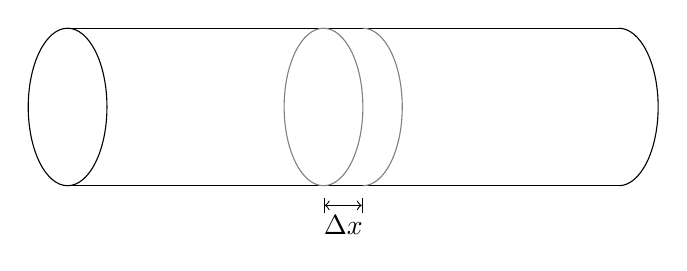
\begin{tikzpicture}
\draw (0,0) circle [x radius=0.5, y radius=1];
\draw (0,-1) -- (7,-1);
\draw (0,1) -- (7,1);
\draw (7,-1) arc [x radius=0.5, y radius=1, start angle=-90, end angle = 90];
\draw[gray] (3.25,0) circle [x radius=0.5, y radius=1];
\draw[gray] (3.75,-1) arc [x radius=0.5, y radius=1, start angle=-90, end angle = 90];

\draw[|<->|] (3.25,-1.25) -- (3.75,-1.25) node [midway, below] {$\Delta x$};
\end{tikzpicture}
\end{center}

The small segment of rod has heat flux $Q(x,t)$ entering in the left side and has heat flux $Q(x+\Delta x,t)$ exiting the right side. The temperature is $T(x,t)$ on the left and $T(x+\Delta x,t)$ on the right.

\begin{center}
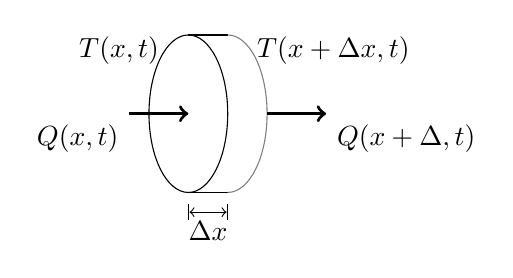
\begin{tikzpicture}

\draw (3.25,1) -- (3.75,1);
\draw (3.25,-1) -- (3.75,-1);
\draw[gray] (3.75,-1) arc [x radius=0.5, y radius=1, start angle=-90, end angle = 90];
\draw(3.25,0) circle [x radius=0.5, y radius=1];

\draw (3,0.5) node [above left] {$T(x,t)$};

\draw[->,very thick] (2.5,0) node [below left] {$Q(x,t)$} -- (3.25,0);

\draw (4,0.5) node [above right] {$T(x+\Delta x,t)$};

\draw[->,very thick] (4.25,0)  -- (5,0) node [below right] {$Q(x+\Delta,t)$};



\draw[|<->|] (3.25,-1.25) -- (3.75,-1.25) node [midway, below] {$\Delta x$};
\end{tikzpicture}
\end{center}

Next, we consider the amount of heat in the segment.  The heat is proportional to both the mass of the segment ($\rho \Delta x$) and the temperature.  The proportionality constant, $c$ is called the specific heat.  The amount of heat in this small segment is:
%
\begin{align*}
c \rho T \Delta x
\end{align*}

The temporal change in heat of this element is the derivative with respect to $t$ and the only quantity that depends on time is the temperature $T$:
%
\begin{align*}
c \rho \frac{\partial T}{\partial t} \Delta x
\end{align*}
and is equal to the amount of heat entering, which is $Q(x,t)$ minus the amount of heat leaving or $Q(x+\Delta x,t)$.
%
\begin{align*}
c \rho \frac{\partial T}{\partial t} \Delta x   = Q(x,t) - Q(x+\Delta x,t)
\end{align*}

Divide both sides of this equation by $\Delta x$ and take the limit $\Delta x \rightarrow 0$,
%
\begin{align}
c \rho \frac{\partial T}{\partial t}    = \lim_{\Delta x \rightarrow 0} Q(x,t) - Q(x+\Delta x,t)
 =   -\frac{\partial Q}{\partial x} \label{eq:heat:eqn:deriv}
\end{align}

The relationship between the heat flux, $Q$ and the temperature is called \emph{Fourier's Law}\index{Fourier's Law}, and states that the heat transferred across unit area is proportional to the temperature gradient or
%
\begin{align*}
Q & = -k \frac{\partial T}{\partial x}
\end{align*}
where $k$ is the proportionality constant called the thermal conductivity and the negative sign is due to the fact that heat flows from hot to cold (in a negative direction).  Substituting Fourier's Law into (\ref{eq:heat:eqn:deriv}) results in
%
\begin{align*}
c \rho \frac{\partial T}{\partial t}  &= -\frac{\partial }{\partial x} \biggl(  -k \frac{\partial T}{\partial x} \biggr)
\end{align*}
and assuming that $k$ is a constant,
\begin{align*}
c \rho \frac{\partial T}{\partial t}& = k \frac{\partial^2 T}{\partial {x}^2} \intertext{rearranging we get}
\frac{\partial T}{\partial t} & = \kappa \frac{\partial^2 T}{\partial {x}^2}
\end{align*}
where $\kappa = k/c \rho$ is called the thermal diffusivity.


\begin{Boxed*}
The \textbf{one-dimensional heat equation} is
%
\begin{align*}
\frac{\partial T}{\partial t} & = \kappa \frac{\partial^2 T}{\partial {x}^2}
\end{align*}
%
and is typically solved for a given initial condition $T(x,0)=f(x)$ and often with boundary conditions.

\end{Boxed*}





\subsection{Wave Equation: Modeling a Taut String}

Next, we turn to modeling the motion of a taut string fixed on both ends.  A common example of this is a guitar string.  We look at a small part of the string that has been displaced vertically from rest:

\begin{center}
\begin{tikzpicture}[scale=1.5]
\draw[<->,thick] (-1,-1) node [below left] {$\vec{T}$} -- (0,0) node [below right] {$u(x,t)$} .. controls (0.5,0.5) and (1,0.75) .. (1.5,1) node [below right] {$u(x+\Delta x,t)$} -- (2.5,1.5) node [right] {$\vec{T}'$} ;
\fill (0,0) circle [radius=2pt];
\fill (1.5,1) circle [radius=2pt];
\end{tikzpicture}
\end{center}
%
where $u(x,t)$ be the vertical position of the string at position $x$ and time $t$ and the tension at $x$ and $x+\Delta x$ are the force vectors $\vec{T}$ and $\vec{T}'$.

To determine an equation that describes the motion of the string, we need to balance the horizontal a vertical forces.  We can write the two force vectors $\mathbf{T}$ and $\mathbf{T}'$ in terms of the horizontal and vertical components where the subscripts in this case are the components as shown in the figure below.

\begin{center}
\begin{tikzpicture}[scale=2]
\draw[<->,thick] (-1,0) node [left] {$\vec{T}_x$} -- (0,0) node [below right] {$u(x,t)$} .. controls (0.5,0.5) and (1,0.75) .. (1.5,1) node [below right] {$u(x+\Delta x,t)$} -- (2.5,1) node [above right] {$\vec{T}'_x$} ;
\fill (0,0) circle [radius=1pt];
\fill (1.5,1) circle [radius=1pt];
\draw[->,thick] (1.5,1) --(1.5,1.5) node [above right] {$\vec{T}'_y$};
\draw[->,thick] (0,0) -- (0,-1) node [below left] {$\vec{T}_y$};
\draw[->,dashed] (0,0) -- (-1,-1);
\draw (-0.2,0) arc [start angle = 180, end angle=225, radius=0.2] node [left] {$\alpha$};

\draw[->, dashed] (1.5,1) -- (2.5,1.5);
\draw (1.7,1) arc [start angle = 0, end angle = {atan(0.5)}, radius=0.2] node [right] {$\beta$};
\end{tikzpicture}
\end{center}

And recall that using Newton's 2nd law of motion the sum of the forces on a object is equal to the mass of the object times its acceleration in that direction or $\sum F = ma$.  There is no horizontal motion of the string, so the horizontal acceleration is zero and therefore:
%
\begin{align}
-\vec{T}_x +\vec{T}'_x & = 0 \notag \\
-||\vec{T}|| \cos \alpha + || \vec{T}'|| \cos \beta & = 0  \notag
\intertext{and solving for $||\vec{T}'||$}
||\vec{T}'|| & = ||\vec{T}|| \frac{\cos \alpha}{\cos \beta}
\label{eq:wave:eqn:derive}
\end{align}

Next, we examine the vertical forces.  The main difference is that there is a vertical acceleration which is the 2nd derivative of the position $u$ with respect to $t$.

\begin{align*}
\sum F & = ma \\
-\vec{T}_y + \vec{T}_y' & = ma \\
-||\vec{T}||\sin \alpha + ||\vec{T}'|| \sin \beta & = \rho \Delta x \frac{\partial^2 u}{\partial {t}^2}
\end{align*}
where the mass of the short piece is $\rho$ the mass density of the string and $\Delta x$ is the horizontal length of the piece.

Substituting (\ref{eq:wave:eqn:derive}) into the equation above,
%
\begin{align*}
-||\vec{T}||\sin \alpha + ||\vec{T}|| \frac{\cos \alpha}{\cos \beta} \sin \beta & = \rho \Delta x \frac{\partial^2 u}{\partial {t}^2}
\intertext{and dividing through by $||\vec{T}|| \cos \alpha$}
-\frac{\sin \alpha}{\cos \alpha} + \frac{\sin \beta}{\cos \beta} & = \frac{\rho \Delta x}{||\vec{T}|| \cos \alpha} \frac{\partial^2 u}{\partial {t}^2} \\
-\tan \alpha + \tan \beta  & = \frac{\rho \Delta x}{||\vec{T}|| \cos \alpha} \frac{\partial^2 u}{\partial {t}^2} \\
\end{align*}

The tangent of the angles are the slopes of the function $u(x,t)$ at $x+\Delta x$ and $x $ respectively, or $\frac{\partial u}{\partial x}$ at $x+\Delta x$ and $x$ therefore the above can be written
%
\begin{align*}
\frac{\partial u}{\partial x} \biggr\vert_{x+\Delta x} - \frac{\partial u}{\partial x}  \biggr\vert_x & = \frac{\rho \Delta x}{||\vec{T}|| \cos \alpha} \frac{\partial^2 u}{\partial {t}^2}  \intertext{Divide by $\Delta x$ and let $T=||\vec{T}|| \cos \alpha$ be the horizontal tension in the string}
\frac{1}{\Delta x} \biggl( \frac{\partial u}{\partial x} \biggr\vert_{x+\Delta x} - \frac{\partial u}{\partial x}  \biggr\vert_x \biggr) & = \frac{\rho}{T} \frac{\partial^2 u}{\partial {t}^2}
\intertext{take the limit as $\Delta x \rightarrow 0$}
\frac{\partial^2 u}{\partial {x}^2}  & = \frac{\rho}{T} \frac{\partial^2 u}{\partial {t}^2}
\end{align*}
The parameter $\rho/T$ plays an important role in the solution, and we'll define $c=\sqrt{T/\rho}$, so the equation can be written:
\begin{align} \label{wave:eqn}
\frac{\partial^2 u}{\partial {t}^2} & = c^2 \frac{\partial^2 u}{\partial {x}^2}
\end{align}

Typically, (\ref{wave:eqn}) is called the \textbf{wave equation} or since there is once one spatial variable, the \textbf{one-dimensional wave equation}.  The remainder of this chapter discusses solutions of the wave equation and related equations.


\section{Linear ordinary differential equations}

As discussed in section \ref{sect:part:deriv:diff:eqns}, a differential equation is linear if it is linear in its dependent variable and derivatives of the dependent variable.  Let's assume that $y$ is the dependent variable and $x$ is the independent variable.  The most general $n$th order ordinary linear differential equation as the form:
%
\begin{align} \label{eq:ODE:linear}
a_n(x) y^{(n)} + a_{n-1}(x) y^{(n-1)} + \cdots + a_1(x) y' + a_0 (x) y = f(x)
\end{align}

In the most general terms, this differential equation is very difficult to solve despite being linear.  However, there are cases when this has nice solutions.  For the most part, we'll look at such equations in this section.

\subsection{Second-order Constant-Coefficient Homogeneous differential equations. }

The most important ordinary differential equations that arise from solving the wave and heat equation are 2nd-order constant coefficient homogeneous differential equations.  If $f(x) \equiv 0$ in (\ref{eq:ODE:linear}), then it is called homogeneous and if the coefficients of the $y$ terms and its derivatives are not dependent on $x$, then the equation is constant-coefficient.  A general 2nd-order ODE with these characteristics can be written:
%
\begin{align*}
a y'' + b y' + cy & = 0
\end{align*}
where $a,b,c$ are real constants.  To solve these, if we let $y=e^{rx}$ and substitute this into the ODE,
%
\begin{align*}
ar^2 e^{rx} + br e^{rx} + ce^{rx} & = 0 \\
e^{rx}(ar^2 + br +c) & = 0 \intertext{and since $e^{rx}$ is never 0}
ar^2+br+c=0
\end{align*}
is called the \textbf{characteristic equation} related to the ODE.  In general, there are two solutions to this equation, $r_1$ and $r_2$.  The general solution to the equation will thus be
%
\begin{align*}
y & = c_1 e^{r_1 x} + c_2 e^{r_2 x}
\end{align*}




\begin{example}  \label{ex:solution:DE:image}
Find the general solution to
%
\begin{align*}
y'' + 3y' + 2y & = 0
\end{align*}

\solution

The characteristic equation is
%
\begin{align*}
r^2 + 3r+2 & = 0 \\
(r+2)(r+1) & = 0
\end{align*}
which has solutions $r=-2$ and $r=-1$.  The general solution thus is
%
\begin{align*}
y & = c_1 e^{-2x} + c_2 e^{-x}
\end{align*}

\end{example}

To find the values of $c_1$ and $c_2$ in the example above or any other differential equation, additional information must be given.  This is analogous to using a point to find the integration constant from an indefinite integral.  The information is generally framed in the language of initial conditions and initial value problems as defined below.

\begin{definition}
A differential equation has \textbf{initial conditions} if at some point $t_0$, then $y(t_0)$, $y'(t_0)$, \ldots, $y^{(n-1)}(t_0)$ are known, where $n$ is the order of the differential equation.  The differential equation together with the initial conditions is known as a \textbf{initial value problem}.
\end{definition}


The next example shows how to fully solve an initial value problem:

\begin{example}
Find the solution to the initial value problem
%
\begin{align*}
y''+3y'+2y & = 0 \qquad \text{$y(0)=3, y'(0) = -4$. }
\end{align*}

\solution

To solve the initial value problem we first solve the differential equation, and this was done in example \ref{ex:solution:DE:image}.  And the general solution is
%
\begin{align} \label{eq:ivp:ex1}
y & = c_1 e^{-2x} + c_2 e^{-x}
\end{align}

Since the initial conditions include knowing the derivative, we will need
%
\begin{align} \label{eq:ivp:ex2}
y' & = -2c_1 e^{-2x} -c_2 e^{-x}
\end{align}
and then we will substitute $y(0)=3$ into (\ref{eq:ivp:ex1}) and $y'(0)=-4$ into (\ref{eq:ivp:ex2}) or
%
\begin{align*}
3 & = c_1 + c_2 \\
-4 & = -2c_1 -c_2
\end{align*}
and the solution to this is $c_1=1$ and $c_2=2$.  Therefore the solution to the initial value problem is
%
\begin{align*}
y & = e^{-2x} + 2e^{-x}
\end{align*}

\end{example}

The next example shows a differential equation that we will see often in this chapter.


\begin{example}
Find the general solution to  $y'' + 9y=0$.

\solution

The characteristic equation is
%
\begin{align*}
r^2+9 & = 0 \\
r & = \pm 3i
\end{align*}
Thus the general solution is
%
\begin{align*}
y & = c_1 e^{3i x} + c_2 e^{-3ix}
\end{align*}

However, we will use Euler's Formula:
%
\begin{align*}
e^{ki\theta} & = \cos k\theta + i \sin k\theta
\end{align*}
to write the equation as a real function:

\begin{align*}
y & = c_1 (\cos 3x + i \sin 3x) + c_2 (\cos 3x - i \sin 3x) \\
& = (c_1+c_2) \cos 3x + (ic_1 - ic_2) \sin 3x  \intertext{letting $C_1 = c_1 + c_2$, $C_2 = ic_1-ic_2$}
y & = C_1 \cos 3x + C_2 \sin 3x
\end{align*}

\end{example}

The characteristic equation for this next example has complex roots.

\begin{example}
Find the solution to $y'' + 4y' +5y=0$.

\solution

The characteristic equation for this differential equation is
%
\begin{align*}
r^2 + 4r + 5 & = 0
\end{align*}
and since this can't be factored, we'll use the quadratic equation to solve this:
%
\begin{align*}
r & = \frac{-4 \pm \sqrt{16-20}}{2} = -2 \pm i
\end{align*}
and  using $y=e^{rx}$ the general solution to this would be written
%
\begin{align*}
y & = c_1 e^{(-2 + i)x} + c_2 e^{(-2-i)x}\\
& = e^{-2x} (c_1 e^{ix} + c_2 e^{-ix}) \\
& = e^{-2x} \bigl( c_1 (\cos x + i \sin x) + c_2 (\cos x - i \sin x) \bigr) \\
& = e^{-2x} \bigl( C_1 \cos x + C_2 \sin x \bigr)
\end{align*}
where $C_1 = c_1+c_2$ and $C_2 = i (c1-c_2)$.
\end{example}

\begin{lemma} \label{lem:soln:2nd:order:DE:homo}
Consider the general 2nd-order constant-coefficient linear homogeneous differential equation,
%
\begin{align} \label{eq:general:2nd:order:DE:homo}
a y'' + b y' + c y & = 0
\end{align}
and let $r_1$ and $r_2$ be the roots of the characteristic equation.
\begin{enumerate}
\item If $r_1$ and $r_2$ are real and distinct, then the general solution to (\ref{eq:general:2nd:order:DE:homo}) is
%
\begin{align} \label{eq:soln:2nd:order:DE:homo:eq1}
y & = c_1 e^{r_1 x} + c_2 e^{r_2 x}
\end{align}
\item If $r_1=r_2$ is the only real root of the characteristic equation then the general solution to (\ref{eq:general:2nd:order:DE:homo}) is
%
\begin{align} \label{eq:soln:2nd:order:DE:homo:eq2}
y & = e^{r_1 x} (c_1 + c_2 x )
\end{align}
\item If the roots of the characteristic equation are pure imaginary, that is $r_1=\beta i$ and $r_2=-\beta i$, then the solution to (\ref{eq:general:2nd:order:DE:homo}) is
%
\begin{align} \label{eq:soln:2nd:order:DE:homo:eq3}
y & = c_1 \sin \beta x + c_2 \cos \beta x
\end{align}
\item and if the roots of the characteristic equation are complex conjugates, that is $r_1=\alpha + \beta i $ and $r_1=\alpha - \beta i $, then the solution to (\ref{eq:general:2nd:order:DE:homo}) is
%
\begin{align} \label{eq:soln:2nd:order:DE:homo:eq4}
y & = e^{\alpha x} \bigl( c_1 \sin \beta x + c_2 \cos \beta x)
\end{align}
\end{enumerate}
\end{lemma}

\begin{proof}
First, recall that the characteristic equation of (\ref{eq:general:2nd:order:DE:homo}) is
%
\begin{align}
a r^2 + br+c & = 0
\end{align}


We will prove each statement in order.

\begin{enumerate}
\item The derivatives of (\ref{eq:soln:2nd:order:DE:homo:eq1}) are
%
\begin{align*}
y' & = c_1 r_1 e^{r_1 x} + c_2 r_2 e^{r_2 x} \\
y'' & = c_1 r_1^2 e^{r_1 x} + c_2 r_2^2 e^{r_2 x}
\end{align*}
and substituting these into (\ref{eq:general:2nd:order:DE:homo}),
%
\begin{align*}
a y'' + b y' + c y & =
a (c_1 r_1^2 e^{r_1 x} + c_2 r_2^2 e^{r_2 x}  ) + b(c_1 r_1 e^{r_1 x} \\
& \qquad + c_2 r_2 e^{r_2 x}) + c(c_1 e^{r_1 x} + c_2 e^{r_2 x})
\intertext{rearranging} \\
 & =  c_1 (a r_1^2 + b r_1 + c) e^{r_1 x} + c_2 (a r_2^2 + b r_2 + c) e^{r_2 x}
 \intertext{and since $r_1$ and $r_2$ are roots of the characteristic equation, then both terms in parentheses are zero and} \\
a y'' + b y' + c y & =  0
\end{align*}
\item The derivatives of (\ref{eq:soln:2nd:order:DE:homo:eq2}) are
%
\begin{align*}
y' & = e^{r_1 x} (r_1 c_1 + c_2 + r_1 c_2  x ) \\
y'' & = e^{r_1 x} (r_1^2 c_1 + 2 r_1 c_2 + r_1^2 c_2 x)
\end{align*}
where the product rule has been used.   In this case, recall also that since $r_1$ is the only real root, that $r_1 = -b/(2a)$ from the quadratic formula with the discriminant $b^2-4ac=0$.  Substituting into (\ref{eq:general:2nd:order:DE:homo})
%
\begin{align*}
a y'' + by' + cy & = a e^{r_1 x} (r_1^2 c_1 + 2 r_1 c_2 + r_1^2 c_2 x) \\
 &  \qquad + be^{r_1 x} (r_1 c_1 + c_2 + r_1 c_2  x ) + c (c_1 + c_2 x )e^{r_1 x} \\
& = \bigl( c_1 (a r_1^2 + b r_1 + c) + c_2 (2 a r_1 + b) \\
& \qquad \qquad + c_2 x (a r_1^2  + br_1  + c)) \bigr) e^{r_1 x}  =0\\
\end{align*}
where the term with factor $c_1$  and the term with factor $c_2 x$ are each 0, because $r_1$ is a root of the characteristic equation.  Lastly, the term with factor $c_2$ is 0 because as stated about $r_1=-b/(2a)$.

\item Note that since the roots are pure imaginary, then then $b=0$ in (\ref{eq:general:2nd:order:DE:homo}) and therefore $r_1$ and $r_2$ satisfy $r^2=-c/a$ and since $r_1=\beta i$, then $\beta^2=c/a$.  The derivatives of (\ref{eq:soln:2nd:order:DE:homo:eq3}) are

\begin{align*}
y' & = c_1 \beta \cos \beta x - c_2 \beta \sin \beta x \\
y'' & = - c_1 \beta^2 \sin \beta x  -c_2 \beta^2 \cos \beta x
\end{align*}
and then substituting into (\ref{eq:general:2nd:order:DE:homo}) with $b=0$,
%
\begin{align*}
ay'' + c y & = a (-c_1 \beta^2 \sin \beta x - c_2 \beta^2 \cos \beta x)  + c ( c_1 \sin \beta x  +c_2 \cos \beta x ) \\
& = c_1 (-a\beta^2  + c) \sin \beta x + c_2 (-a\beta^2 +c) \cos \beta x =0
\end{align*}
since $\beta^2=c/a$.



\item In this case, since the roots are complex conjugates, we can write $r_1=\alpha+i\beta $ and $r_2=\alpha-i\beta$.  The characteristic equation can be written:
%
\begin{align*}
a(r-r_1)(r-r_2) & = a(r-(\alpha + i \beta))(r-(\alpha-i\beta)) \\
& = a r^2 - 2 a \alpha r + a(\alpha^2+\beta^2) = 0
\end{align*}
which implies that $b=-2a \alpha$ and $c=a(\alpha^2+\beta^2)$.
The derivatives of (\ref{eq:soln:2nd:order:DE:homo:eq4}) are
%
\begin{align*}
y' & = e^{\alpha x} \bigl( (c_1 \alpha - c_2 \beta) \sin \beta x + (c_2 \alpha + c_1 \beta) \cos \beta x) \bigr) \\
y'' & = e^{\alpha x} \bigl( (c_1 \alpha^2 -2 c_2 \alpha \beta - c_1 \beta^2) \sin \beta x \\
& \qquad \qquad + (c_2 \alpha^2 + 2 c_1 \alpha \beta - c_2 \beta^2) \cos \beta x\bigr)
\end{align*}
and substituting them into (\ref{eq:general:2nd:order:DE:homo}),
%
\begin{align}
a y'' + by' + cy & = a e^{\alpha x} \bigl( (c_1 \alpha^2 -2 c_2 \alpha \beta - c_1 \beta^2) \sin \beta x   \notag \\
& \qquad \qquad + (c_2 \alpha^2 + 2 c_1 \alpha \beta - c_2 \beta^2) \cos \beta x\bigr) \notag \\
& \qquad + b e^{\alpha x} \bigl( (c_1 \alpha - c_2 \beta) \sin \beta x + (c_2 \alpha + c_1 \beta) \cos \beta x) \bigr)  \notag \\\
& \qquad + c e^{\alpha x} \bigl( c_1 \sin \beta x + c_2 \cos \beta x) \notag \\\
& = e^{\alpha x} \bigl ( c_1 (a\alpha^2-a\beta^2 +b\alpha + c) \sin \beta x   \notag \ \\
& \qquad + c_1 (2a\alpha\beta+b\beta) \cos \beta x + c_2 (-2a\alpha \beta-b\beta) \sin \beta x   \notag \\\
& \qquad + c_2 (a \alpha^2 - a \beta^2 + b \alpha + c) \bigr)  \label{eq:soln:2nd:order:DE:homo:eq4:proof}
\end{align}
And using $b=-2a\alpha$ and $c=a(\alpha^2+\beta^2)$, the right hand side of (\ref{eq:soln:2nd:order:DE:homo:eq4:proof}) is 0, therefore
(\ref{eq:soln:2nd:order:DE:homo:eq4}) is a solution.

\end{enumerate}

~
\end{proof}






\subsection{Solutions to Ordinary Differential Equations as Vector Spaces}

We studied vector spaces in section \ref{sect:vector:space} and a common example of a vector space that is not $\mathbb{R}^n$ is that of functions.  It can be shown that the set related to the differential equation in Example \ref{ex:solution:DE:image}
%
\begin{align*}
V & = \{ y \in \mathcal{C}^{(2)}(\mathbb{R}) \; | \; y'' + 9 y = 0 \}
\end{align*}
is a vector space or a subspace of $\mathcal{C}^{(2)}$, the vector space of all functions with continuous 2nd derivatives.  The basis of the subspace are the two solutions of the differential equation or $B=(\cos 3x, \sin 3x)$.  Note that the general solution to the differential equation is the linear combination of the basis vectors or the span of the two solutions.



\section{Sturm-Liouville Problems }  \label{sect:sturm:liouville}

We now turn to a class of differential equations that arise in solving partial differential equations.  This class is called Sturm-Liouville problems and they satisfy boundary conditions instead of the initial conditions that we saw in the previous section.

\begin{definition}
Consider the differential equation
%
\begin{align*}
[r(x) y']' + [p(x) + \lambda q(x)] y & = 0
\end{align*}
for $r(x), p(x) \in \mathcal{C}^{(1)[a,b]}$, $q(x)\in \mathcal{C}^{(0)}[a,b]$, and $\lambda \in \mathbb{R}$.  The differential equation is also subject to the boundary conditions:
\begin{align*}
a_1 y(a) + a_2 y'(a) & = 0 \\
b_1 y(b) + b_2 y'(b) & = 0
\end{align*}
such that both $a_1$ and $a_2$ cannot be zero as well as both $b_1$ and $b_2$.

The differential equation with these boundary conditions are called a \textbf{Sturm-Liouville Problem}.  The solution is called an \textbf{eigenfunction} of the problem and the values of $\lambda$ are called the \textbf{eigenvalues}.

\end{definition}

The following example shows how to solve a Sturm-Liouville problem, that is, find the eigenvalues and eigenfunctions of the problem.

\begin{example} \label{ex:sturm:liouville}
Find the eigenvalue and eigenfunctions of the Sturm-Liouville problem:
\begin{align*}
y''+\lambda y & = 0 & y(0) & = y(L)  = 0
\end{align*}

\solution

First note that $r(x)=q(x) \equiv 1$ and also $a_1=b_1=1$ and $a_2=b_2=0$, which satisfies the conditions on the boundaries.

The characteristic equation for this problem is:
%
\begin{align*}
r^2+\lambda & = 0
\end{align*}
which has the solutions $r = \pm \sqrt{-\lambda}$.  The form of the equation depends on $\lambda$.  If $\lambda=0$, we get:
%
\begin{align} \label{eq:sturm:liouville:ex:eq1}
y & = A + B x
\end{align}
if $\lambda<0$, then the solution is
%
\begin{align} \label{eq:sturm:liouville:ex:eq2}
y & = c_1 e^{\sqrt{-\lambda} x} + c_2 e^{-\sqrt{-\lambda} x}
\end{align}
and if $\lambda>0$, then we get
%
\begin{align} \label{eq:sturm:liouville:ex:eq3}
y & = C_1 \cos \sqrt{\lambda} x + C_2 \sin \sqrt{\lambda} x
\end{align}

Next, we apply the boundary conditions on all three solutions.  Recall that $y(0)=y(L)=0$.

If $\lambda = 0$, substituting the boundary conditions into (\ref{eq:sturm:liouville:ex:eq1}),
%
\begin{align*}
A+ B(0)& = 0 && \text{so $A=0$} \\
A+B(L) & = 0 && \text{so $B=0$}
\end{align*}
so the only solution to (\ref{eq:sturm:liouville:ex:eq1}) is the trivial solution $y\equiv 0$.

If $\lambda >0$, then substituting the boundary conditions into (\ref{eq:sturm:liouville:ex:eq2}) results in
\begin{align*}
c_1 (1) + c_2(1) & = 0 \\
c_1(e^{\sqrt{-\lambda} L} + c_2 e^{-\sqrt{-\lambda} L}) & = 0
\end{align*}
From the first equation, $c_1=-c_2$ and substituting this into the 2nd equation
%
\begin{align*}
c_1 e^{\sqrt{-\lambda} L} - c_1 e^{-\sqrt{-\lambda} L} & = 0 \\
c_1 e^{\sqrt{-\lambda}L} \bigl( 1- e^{-2\sqrt{-\lambda} L}) & = 0
\end{align*}
$c_1=0$ is a solution, the second term is never zero and the third term is only zero if $L=0$, which is not true or $\lambda=0$, which is also not true, since this case is $\lambda >0$.  Therefore again, the only solution to (\ref{eq:sturm:liouville:ex:eq2}) is the trivial solution.

If $\lambda<0$ then substituting the boundary conditions into (\ref{eq:sturm:liouville:ex:eq3}) results in
%
\begin{align*}
C_1 (1) + C_2 (0) & = 0 && \text{so $C_1=0$} \\
(0) \cos \sqrt{\lambda} L + C_2 \sin \sqrt{\lambda} L = 0
\end{align*}
the second states that either $C_2=0$, again the trivial solution or
%
\begin{align*}
\sin \sqrt{\lambda} L & = 0
\end{align*}
which occurs if $\sqrt{\lambda} L = n \pi$ for $n=0,\pm 1, \pm 2, \pm 3, \ldots$.   Or
%
\begin{align} \label{eq:sturm:liouville:ex:eigs}
\lambda = \frac{n^2 \pi^2}{L^2}
\end{align}
We now check which values of $n$ result in valid values of $\lambda$.

When $n=0$, we get $\lambda=0$ again, which violates $\lambda<0$ and for $n$ both plus and minus the same number, we get the same eigenvalue, so we will discard the negative values of $n$ and just include $n=1,2,3, \ldots. $

The eigenvalues of this problem are those in (\ref{eq:sturm:liouville:ex:eigs}) for $n=1,2,3,\ldots$and the eigenfunctions of this problem are:
%
\begin{align*}
\phi_n(x) & = \sin \frac{n\pi x}{L}
\end{align*}

\end{example}

It may have appears that we were lucky that there was a solution to the Sturm-Liouville problem in the above example.  However, this is not the case and any Sturm-Liouville problem has a solution as the following theorem shows.


\begin{theorem} \label{thm:sturm:liouville}
Let $\lambda_n$ and $\phi_n(x)$ be any eigenvalue and eigenfunction of the Sturm Liouville problem.
\begin{enumerate}
\item The eigenvalue $\lambda_n$ is real.
\item There are an infinite number of eigenvalues that can be ordered $\lambda_1 < \lambda_2< \lambda_3 < \cdots $ and for each eigenvalue, there is only one eigenfunction.
\item Eigenfunctions $\phi_n$ and $\phi_m$ with $\lambda_n \neq \lambda_m$ satisfy $\langle \phi_n , \phi_m \rangle = 0$.
\item Let $f$ and $f'$ be piecewise continuous functions on $[a,b]$.  If
\begin{align*}
a_n = \frac{\langle f,\phi_n \rangle }{ \langle \phi_n, \phi_n \rangle},
\end{align*}
then the series:
%
\begin{align*}
\sum_{n=1}^{\infty}a_n \phi_n(x)
\end{align*}
converges to $f$ if $f$ is continuous at $x$ and to the value $(f(x+)+f(x-))/2$ if $f$ is discontinuous at $x$ for each point in $[a,b]$.
\end{enumerate}
\end{theorem}

\begin{example}
Let $f(x)=x$ on $[0,L]$.  Find the series expansion listed in the theorem corresponding to the Sturm-Liouville problem $y''+\lambda y= 0$.

\solution

\begin{align*}
a_n & = \frac{ \langle f,\phi_n \rangle}{ \langle \phi_n, \phi_n \rangle} \\
& = \frac{1}{L/2} \int_{0}^L f(x) \sin \frac{n\pi x}{L} \, dx
\end{align*}
which is the Fourier sine series.

\end{example}


\begin{example} \label{ex:sturm:liouville:2}
Find the solution of the Sturm-Liouville problem
%
\begin{align*}
y'' + \lambda y &= 0 & y'(0) = 0, && y'(L) & = 0
\end{align*}

\solution

Since this the same differential equation as in Example \ref{ex:sturm:liouville}, we note that when $\lambda>0$, there was no solution and the same is true here.  In the case of $\lambda=0$, the solution is
%
\begin{align*}
y & = A+Bx
\end{align*}
and the derivative is needed as well,
%
\begin{align*}
y' & = B
\end{align*}
and then applying the boundary condition $y'(0)=y'(L)=0$, implies that $B=0$, however, $A$ is not determined and $y=A$ is a solution.

Next, we turn to  $\lambda>0$, with the solution,
%
\begin{align*}
y & = C_1 \cos \sqrt{\lambda} x + C_2 \sin \sqrt{\lambda} x
\end{align*}
and again, we need the derivative,
%
\begin{align*}
y' & = - C_1 \sqrt{\lambda} \sin \sqrt{\lambda} x + C_2 \sqrt{\lambda} \cos \sqrt{\lambda} x
\end{align*}
Applying the boundary condition, $y'(0)=0$, results in
%
\begin{align*}
y'(0) & = C_2 \sqrt{\lambda} = 0
\end{align*}
which implies that $C_2=0$.  Applying the boundary condition $y'(L)=0$ results in
%
\begin{align*}
y'(L) & = -C_1 \sqrt{\lambda} \sin \sqrt{\lambda} L = 0
\end{align*}
and if $C_1=0$, this results in the trivial solution, $\lambda$ cannot be zero, however
%
\begin{align*}
\sin \sqrt{\lambda} L & = 0
\end{align*}
when $\sqrt{\lambda} L = n \pi$ or $\lambda = n^2 \pi^2/L^2$.

The eigenvalues and eigenfunctions of this problem then are $\lambda_0 =0$ and $\phi_0=1$, and
%
\begin{align*}
\lambda_n & = \frac{n^2 \pi^2}{L^2} & \phi_n & = \cos \frac{n \pi x}{L}
\end{align*}

\end{example}


There are other Sturm-Liouville problems that arise commonly and we will see others later in this chapter and solve them as they arise.  We will use these solutions that we just found in solving the PDEs that we derived above.

\section[Solving the Wave Equation]{Solving the 1D Wave Equation Using Separation of Variables}

We derived the 1D wave equation in section \ref{sect:modeling:pdes}.  We will now solve this as an initial value problem.  Consider
%
\begin{align*}
\frac{\partial^2 u}{\partial {t}^2} &= c^2 \frac{\partial^2 u}{\partial {x}^2}  \intertext{with boundary conditions}
u(0,t) & = u(L,t) = 0, \qquad \text{for $t \geq 0$} \\
\intertext{and initial conditions}
u(x,0) & = f(x)  \qquad  \text{for $0 \leq x \leq L$ } \\
u_t(x,0) & = 0 \qquad \text{for $0 \leq x \leq L$}
\end{align*}

The technique of \textbf{separation of variables} is the standard way to solve this and other linear PDEs.  First start by assuming that the solution $u(x,t)$ can be written as a product of functions solely of $x$ and $t$ or $u(x,t) = X(x) T(t)$.  Then substituting this into the PDE:
%
\begin{align*}
\frac{\partial^2 (X(x)T(t))}{\partial {t}^2} & = c^2 \frac{\partial^2 (X(x) T(t))}{\partial {x}^2}  \\
XT'' & = c^2 X'' T && \text{dividing by $c^2XT$} \\
\frac{1}{c^2}\frac{T''}{T} & = \frac{X''}{ X}
\end{align*}
Now since $T$ (and therefore $T''$) depends only on $t$ and $X$ (and also $X''$) only depends on $x$, each side of the PDE must be equal to a constant (independent of either $x$ or $t$). Let's say it is $-\lambda$ or
%
\begin{align*}
\frac{1}{c^2} \frac{T''}{T} & = \frac{X''}{X} = -\lambda
\end{align*}
This results in two equations:
%
\begin{align} \label{eq:sep:vars:T}
T'' +c^2\lambda T &= 0
\\ X'' + \lambda X & = 0 \label{eq:sep:vars:X}
\end{align}


The boundary conditions are $u(0) = u(L) = 0$ for all $t$, so substituting $u=XT$ we get
%
\begin{align*}
X(0)T(t) = X(L) T(t) & = 0
\end{align*}
for all $t$ or $X(0)=X(L)=0$.  The ODE for $X$ is that in (\ref{eq:sep:vars:X}) with these boundary conditions.  This is a Sturm-Liouville problem that was solved in example \ref{ex:sturm:liouville}.   We know that the only form of the solution is when $\lambda>0$ and from the problem that we solved above we know that
%
\begin{align} \label{eq:sep:vars:eigenvalues}
\lambda & = \frac{n^2 \pi^2}{L^2}
\end{align}
and the solution for $X$ are the eigenfunctions of the problem:
%
\begin{align*}
X_n(x) & = \sin \frac{n \pi x}{L}
\end{align*}
for $n=1,2,3,\ldots$.

Next, we need to solve (\ref{eq:sep:vars:T}) and using the eigenvalues in (\ref{eq:sep:vars:eigenvalues})
%
\begin{align*}
T'' + c^2 \frac{n^2 \pi^2}{L^2} T = 0
\end{align*}
The solution to this is found by assuming $T(t) = e^{r t}$ and getting the characteristic equation
%
\begin{align*}
r^2 + c^2 \frac{n^2 \pi^2}{L^2} = 0
\end{align*}
and thus
%
\begin{align*}
r & = \pm i \frac{n c \pi}{L}
\end{align*}
and the solution to this is
%
\begin{align*}
T_n(t) & = a_n \cos \biggl( \frac{n c \pi }{L} \biggr) t + b_n \sin \biggl( \frac{n c \pi }{L} \biggr) t
\end{align*}

We know then that the following is a solution to the PDE:
%
\begin{align*}
u_n(x,t) & = X_n(x) T_n(t) = \biggl( a_n \cos \biggl( \frac{n c \pi }{L} \biggr) t + b_n \sin \biggl( \frac{n c \pi }{L} \biggr) t \biggr) \sin \frac{n \pi x}{L}
\end{align*}

The \textbf{principle of superposition} states that a sum of these solutions is also a solution to the original PDE and in fact the most general solution is
%
\begin{align*}
u(x,t) & = \sum_{n=1}^{\infty} u_n(x,t) \\
& = \sum_{n=1}^{\infty} \biggl( a_n \cos \biggl( \frac{n c \pi }{L} \biggr) t + b_n \sin \biggl( \frac{n c \pi }{L} \biggr) t \biggr) \sin \frac{n \pi x}{L}
\end{align*}

Lastly, we use the initial conditions $u(x,0)=f(x)$  and $u_t(x,0)=0$  for $0 \leq x \leq L$ to solve for $a_n$ and $b_n$ above.  We will look at the second condition first:
%
\begin{align*}
u_t(x,t) & = \sum_{n=1}^{\infty} \frac{n c \pi}{L} \biggl( -a_n \sin \biggl( \frac{n c \pi }{L} \biggr) t + b_n \cos \biggl( \frac{n c \pi }{L} \biggr) t \biggr) \sin \frac{n \pi x}{L}
\end{align*}
and evaluated at $t=0$:
%
\begin{align*}
u_t(x,0) &= \sum_{n=1}^{\infty} \frac{n c \pi}{L} \biggl( 0 + b_n \biggr) \sin \frac{n \pi x}{L}
\end{align*}
and since $u_t(x,0)\equiv 0$, then $b_n=0$.  The first condition:
%
\begin{align*}
u(x,0) & = f(x) = \sum_{n=1}^{\infty}  a_n \sin \frac{n \pi x}{L}
\end{align*}
is the Fourier sine series for $0 \leq x \leq L$.   Thus
%
\begin{align*}
a_n & = \frac{2}{L} \int_{0}^L f(x) \sin \frac{n \pi x}{L} \, dx
\end{align*}

We summarize the solution to the wave equation.

\begin{Boxed*}
The solution to the wave equation
%
\begin{align*}
u_{tt} =c^2 u_{xx}
\end{align*}
with boundary conditions
%
\begin{align*}
u(0,t)& = u(L,t) = 0
\end{align*}
and initial conditions
\begin{align*}
u(x,0) & = f(x), \\
u_t(x,0) & = 0
\end{align*}
is
\begin{align*}
u(x,t) & = \sum_{n=1}^{\infty}  a_n \cos \biggl( \frac{n c \pi }{L} \biggr) t  \sin \frac{n \pi x}{L}
\end{align*}
where
%
\begin{align*}
a_n & = \frac{2}{L} \int_0^L f(x) \sin \frac{n\pi x}{L} \, dx
\end{align*}
\end{Boxed*}

\bigskip

The following two examples show specific solutions for given functions $f(x)$.



\begin{example}
Find the specific solution to the wave equation if $f(x) = 0.1 \sin (\pi x/L)$

\solution

Specifically, we only need to find the coefficients $a_n$ above:

\begin{align*}
a_n & = \frac{2}{L} \int_0^L 0.1 \sin \frac{\pi x}{L}  \sin \frac{n\pi x}{L}  \, dx \\
& = \begin{cases}
0.1 \qquad \text{if $n=1$} \\
0 \qquad \text{otherwise}
\end{cases}
\end{align*}
Thus the full solution to the PDE is:
%
\begin{align*}
u(x,t) & = 0.1 \sin \frac{\pi x}{L} \cos \frac{\pi t}{L}
\end{align*}
\end{example}


\begin{example}
Find the solution to the wave equation above if the initial shape of the string is
%
\begin{align*}
f(x) & = \begin{cases}
kx,&  \text{if $0\leq x< L/2$} \\
k(L-x),& \text{if $L/2 \leq x \leq L$}
\end{cases}
\end{align*}

As before, we only need to find the coefficients of $a_n$ given by
%
\begin{align*}
a_n & = \frac{2}{L} \int_0^L  f(x)  \sin \frac{n \pi x}{L} \, dx \\
& = \frac{2}{L} \int_0^{L/2} kx \sin \frac{n \pi x}{L} \, dx + \frac{2}{L} \int_{L/2}^L k(L-x) \sin \frac{n \pi x}{L} \, dx \\
& = \begin{cases}
\frac{4k L}{n^2 \pi^2} (-1)^{(n-1)/2} , & \text{if $n$ is odd} \\
0, & \text{otherwise}
\end{cases}
\end{align*}

And thus the full solution to the wave equation is:
%
\begin{align*}
u(x,t) & = \sum_{n=1}^{\infty}a_n \sin \biggl(\frac{n \pi x}{L} \biggr) \sin \biggl(\frac{n \pi t}{L} \biggr)  \\
& = \sum_{n=1}^{\infty} \frac{4 k L (-1)^{n+1}}{\pi^2 (2n-1)^2} \sin \biggl( \frac{(2n-1) \pi x}{L} \biggr)   \sin \biggl(\frac{(2n-1) \pi t}{L} \biggr)
\end{align*}
\end{example}

\subsection{Solution to the Wave Equation with a free boundary condition}

We now look at the wave equation with what is termed a free boundary condition.  Consider
%
\begin{align}
\frac{\partial^2 u}{\partial {t}^2} &= c^2 \frac{\partial^2 u}{\partial {x}^2}  \notag\intertext{with boundary conditions}
u(0,t) & = 0 \qquad u_x(L,t) = 0, \qquad \text{for $t \geq 0$} \label{eq:wave:bc:free}\\
\intertext{and initial conditions}
u(x,0) & = f(x)  \qquad  \text{for $0 \leq x \leq L$ } \label{eq:wave:free:ic1} \\
u_t(x,0) & = 0 \qquad \text{for $0 \leq x \leq L$}  \label{eq:wave:free:ic2}
\end{align}
and the difference between this and the initial value problem at the beginning of the section is the boundary condition at $x=L$.  Above, the function $u$ was forced to be 0 there and in this case, the derivative is 0 at $x=L$.

Using separation of variables by assuming that $u(x,t)=X(x)T(t)$, and substituting into the wave equation and dividing through by $c^2 XT$, we again get the equation
%
\begin{align*}
\frac{1}{c^2} \frac{T''}{T} & = \frac{X''}{X} = -\lambda^2
\end{align*}
where again since each term only depends on $t$ or $x$, it must be a constant, which we say is $-\lambda$.  The differential equation in $X$ is
%
\begin{align*}
X'' + \lambda X & = 0 & X(0)& = 0, X'(L)=0
\end{align*}

where the boundary conditions came from (\ref{eq:wave:bc:free}).  The solution to this Sturm-Liouville problem is similar to those in Examples \ref{ex:sturm:liouville} and \ref{ex:sturm:liouville:2}, however the details of this are not shown. The eigenfunctions and eigenvalues of this are
%
\begin{align*}
X_n(x) & = \sin \lambda_n x & \lambda_n & = \frac{(2n-1)\pi}{2L}
\end{align*}

Next, we seek the solution to $T''+c^2 \lambda^2 T = 0$ which again, similar to solution of the wave equation with fixed boundary conditions, is
%
\begin{align*}
T & = a \cos c \lambda t + b \sin c \lambda t
\end{align*}
which has a solution for each value of $n$ or
%
\begin{align*}
T_n & = a_n \cos c \frac{(2n-1)\pi}{2L} t + b_n \sin c \frac{(2n-1)\pi}{2L} t
\end{align*}

Using the principle of superposition, the sum of solutions is also a solution, so
%
\begin{align} \label{eq:wave:free:eq1}
u(x,t) & = \sum_{n=1}^{\infty} \biggl(a_n \cos c \frac{(2n-1)\pi}{2L} t + b_n \sin c \frac{(2n-1)\pi}{2L} t \biggr) \sin \frac{(2n-1)\pi x}{2L}
\end{align}

To find the particular solution, we need to find the constants $a_n$ and $b_n$ which can be found using the initial conditions of the problem.  Similar to the problem above with the fixed boundary conditions, we will use the initial condition in (\ref{eq:wave:free:ic2}) first, which requires that we know the derivative.  And

\begin{align*}
u_t & = \sum_{n=1}^{\infty} c \lambda_n \biggl(-a_n \sin c \frac{(2n-1)\pi}{2L} t + b_n \cos c \frac{(2n-1)\pi}{2L} t \biggr) \sin \frac{(2n-1)\pi x}{2L}
\end{align*}

Applying the initial condition in (\ref{eq:wave:free:ic2}),
\begin{align*}
u_t(x,0)=0 & = \sum_{n=1}^{\infty}b_n c \lambda_n  \sin \frac{(2n-1)\pi x}{2L}
\end{align*}
which implies that $b_n=0$ for all $n$.  Next, if we substitute this into (\ref{eq:wave:free:eq1}) and apply the boundary condition in (\ref{eq:wave:free:ic1}),
%
\begin{align*}
u(x,0) & = f(x) = \sum_{n=1}^{\infty} a_n \sin \frac{(2n-1)\pi x}{2L}
\end{align*}
and the coefficients can be found using Theorem \ref{thm:sturm:liouville}, to be
%
\begin{align*}
a_n & = \frac{\langle f(x), X_n(x) \rangle}{\langle X_n(x), X_n(x) \rangle} \\
& = \frac{\int_0^L f(x) \sin (2n-1)\pi x/(2L) \, dx }{\int_0^L \sin^2 (2n-1)\pi x/(2L) \, dx } \\
& = \frac{2}{L} \int_0^L f(x) \sin  \frac{(2n-1)\pi x}{2L} \, dx
\end{align*}

\begin{Boxed*}
To summarize, the solution to the 1D wave equation
\begin{align*}
\frac{\partial^2 u}{\partial {t}^2} &= c^2 \frac{\partial^2 u}{\partial {x}^2} \intertext{with boundary conditions}
u(0,t) & = 0 \qquad u_x(L,t) = 0, \qquad \text{for $t \geq 0$} \\
\intertext{and initial conditions}
u(x,0) & = f(x)  \qquad  \text{for $0 \leq x \leq L$ } \\
u_t(x,0) & = 0 \qquad \text{for $0 \leq x \leq L$}
\end{align*}
is
\begin{align}
u(x,t) & = \sum_{n=1}^{\infty} a_n \cos c \frac{(2n-1)\pi}{2L} t  \sin \frac{(2n-1)\pi x}{2L}  \label{eq:wave:free:solution}
\end{align}
where
\begin{align}
a_n & = \frac{2}{L} \int_0^L f(x) \sin  \frac{(2n-1)\pi x}{2L} \, dx
\label{eq:wave:free:fourier:coeffs}
\end{align}

\end{Boxed*}


\begin{example}
Find the solution to the 1D wave equation with free boundary condition at $x=1$ if
%
\begin{align*}
f(x) &= x^2 & &\text{for $0 \leq x \leq 1$}
\end{align*}

\solution

In this case, we only need to find the constants $a_n$ as defined in (\ref{eq:wave:free:fourier:coeffs}),
%
\begin{align*}
a_n & = 2 \int_0^1 x^2 \sin \frac{(2n-1)\pi x}{2} \, dx \\
& = \frac{(-1)^n (8\pi + 16\pi n) -16}{(2n-1)^3 \pi^3}
\end{align*}

So the full solution to this wave equation is
%
\begin{align*}
u(x,t) & = \sum_{n=1}^{\infty} \frac{(-1)^n (8\pi + 16\pi n) -16}{(2n-1)^3 \pi^3} \cos c \frac{(2n-1)\pi}{2L} t  \sin \frac{(2n-1)\pi x}{2L}
\end{align*}

\end{example}


\section{Solution to the 1D Heat Equation}

In this section we will investigate solving the 1D heat equation
%
\begin{align*}
\frac{1}{\kappa} \frac{\partial u}{\partial t}& = \frac{\partial^2 u}{\partial {x}^2}
\end{align*}
with boundary conditions:
%
\begin{align*}
\frac{\partial u}{\partial x} \biggr\vert_{x=0} & = 0 &  \frac{\partial u}{\partial x} \biggr\vert_{x=L} & = 0
\end{align*}
indicating that the end are insulated and the initial condition is:
%
\begin{align*}
u(x,0) = f(x),\quad  \text{if $0 < x < L$ }
\end{align*}

As with the wave equation, we use the technique of separation of variables.  That is let $u=X(x)T(t)$ to get:
%
\begin{align*}
\frac{1}{\kappa} T' X & = T X'' && \text{divide through by $XT$} \\
\frac{1}{\kappa} \frac{T'}{T} & = \frac{X''}{X}
\end{align*}
since the left side only depends on $t$ and the right side only depends on $X$, it must be that these must both equal only a constant, (call it $-\lambda$) therefore we get the two equations:
%
\begin{align*}
\frac{1}{\kappa} \frac{T'}{T} & = -\lambda & \frac{X''}{X} = -\lambda  \intertext{or}
T' + \kappa \lambda T & = 0 & X'' + \lambda X & = 0
\end{align*}
The boundary conditions for the second equation becomes:
%
\begin{align*}
X'(0)=X'(L)=0
\end{align*}
This is a Sturm-Liouville problem that we saw in Example \ref{ex:sturm:liouville:2}  which has the solution:
%
\begin{align*}
\lambda_n & = \frac{n^2 \pi^2}{L^2} \quad \text{$n=0,1,2,\ldots$}  \\
X_n (x) & = \cos \frac{n \pi x}{L}
\end{align*}
if $n>1$ and $\lambda_n=0$ and $X_n = 1$ is also a solution.

The solution to $T'+\kappa \lambda T = 0$ can be found by letting $T= e^{at}$ and substituting in
%
\begin{align*}
a e^{at} + \kappa \lambda e^{at} = e^{at}(a + \kappa \lambda) & = 0
\end{align*}
or
%
\begin{align*}
a = - \kappa \lambda
\end{align*}
therefore the solution is
%
\begin{align*}
T_n & = e^{-\kappa \lambda t} = e^{-(\kappa/L^2) n^2 \pi^2 t}
\end{align*}

A solution $u_n(x,t)$ to the equation is
%
\begin{align*}
u_n(x,t) & = X_n(x,t) T_n(x,t) \\
& = e^{-(\kappa/L^2) n^2 \pi^2 t} \cos \frac{n \pi x}{L}
\end{align*}
and using the principle of superposition the general solution to the PDE with given boundary conditions is:
%
\begin{align*}
u & = \sum_{n=0}^{\infty} C_n e^{-(\kappa/L^2) n^2 \pi^2 t} \cos \frac{n \pi x}{L}
\end{align*}

Next, the initial condition is:
%
\begin{align*}
u(x,0) = f(x) = \sum_{n=0}^{\infty} C_n \cos \frac{n \pi x}{L}
\end{align*}
and the coefficients can be found by the Sturm-Liouville theorem to get:
%
\begin{align*}
C_0 & = \frac{1}{L} \int_0^L f(x) \, dx \\
C_n & = \frac{2}{L} \int_0^L f(x) \cos \frac{ n \pi x}{L} \, dx
\end{align*}


\begin{example}
Find the solution to the heat equation given above if the initial condition is:
%
\begin{align*}
f(x) = 1+\cos \frac{2\pi x}{L}
\end{align*}

\solution

In this case, we need to find $C_0$ and $C_n$:

\begin{align*}
C_0 & = \frac{1}{L} \int_0^L (1+ \cos \frac{2\pi x}{L}) \, dx  = 1 \\
C_n& = \frac{2}{L} \int_0^L \cos \frac{2\pi x}{L} \cos \frac{n \pi x}{L} \, dx \\
& = \begin{cases}
1 & \text{if $n=2$} \\
0 & \text{otherwise}
\end{cases}
\end{align*}
so the solution to the PDE is:
%
\begin{align*}
u(x,t) & = 1 + e^{-(\kappa/L^2) 4 \pi^2 t } \cos \frac{2\pi x}{L}
\end{align*}

To get a feeling for the solution, the following is a plot when $\kappa=0.001$, $L=1$ for $t=0,5,10,15$.


\begin{center}
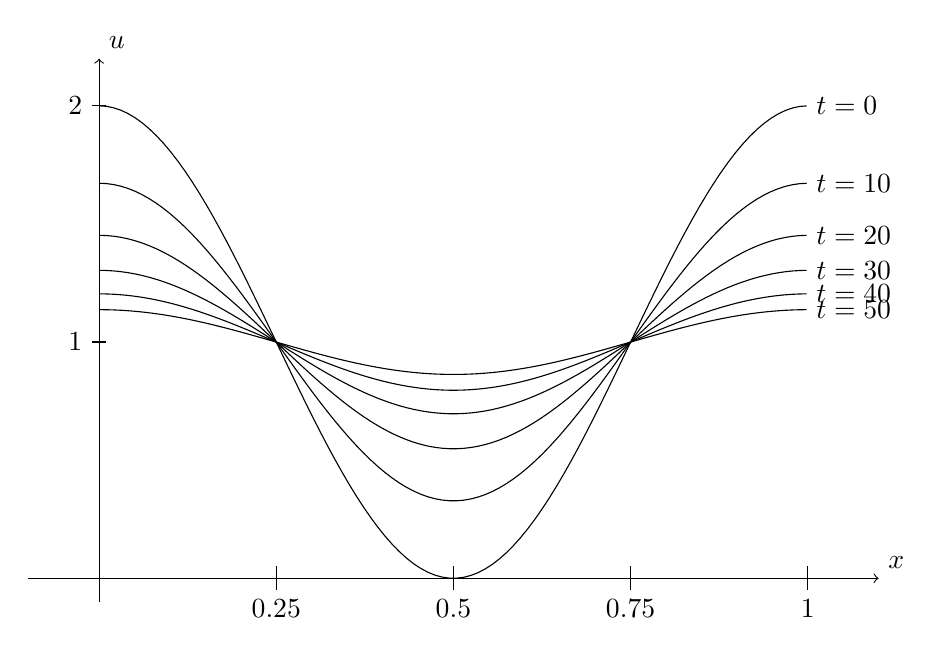
\begin{tikzpicture}[xscale=9,yscale=3]
\draw[->] (-0.1,0) -- (1.1,0) node [above right] {$x$};

\foreach \x in {0.25,0.5,0.75,1} \draw (\x,0.05)--(\x,-0.05) node [below] {\x};
\foreach \y in {1,2} \draw (0.01,\y) -- (-0.01,\y) node [left] {\y};

\draw[->] (0,-0.1) -- (0,2.2) node [above right] {$u$};
\foreach \t in {0,10,...,50}
\draw plot[domain=0:1,samples=100] (\x,{1+exp(-0.001*4*pi*pi*\t)*cos(2*pi*\x r)}) node [right] {$t=\t$};
\end{tikzpicture}
\end{center}

The plot shows the temperature distribution for the initial case $t=0$ and subsequent times.  The temperature evens out as time increases and in the limit the temperature would be 1 throughout, which is the average initial temperature.

\end{example}


\section{Heat Equation in two spatial dimensions}

The Heat equation in 2 spatial dimensions can be written:
%
\begin{align} \label{eq:heat:eqn:2D}
\frac{1}{\kappa} \frac{\partial u}{\partial t} & = \frac{\partial^2 u}{\partial {x}^2}  + \frac{\partial^2 u}{\partial {y}^2}
\end{align}

In this case, let's say that we have the following boundary conditions:
%
\begin{align*}
u\bigr\vert_{x=0} & = 0 & \frac{\partial u}{\partial x}\biggr\vert_{x=L} & = 0 \\
\frac{\partial u}{\partial y} \biggr\vert_{y=0} & = 0 & \frac{\partial u}{\partial y}\biggr\vert_{y = \ell}  &  = 0
\end{align*}
which means that along the edge $x=0$, the temperature is 0 and the other three edges are insulated.  In addition, assume that the initial condition is
%
\begin{align*}
u(x,y,0) & = f(x,y)
\end{align*}

In this section, we will examine how to solve this problem using the separation of variables.  Since there are 3 variables, let's assume that the solution $u$ can be written:
%
\begin{align*}
u & = X(x) Y(y) T(t)
\end{align*}
%
and substituting this into the heat equation, we get:
%
\begin{align*}
\frac{1}{\kappa} \frac{\partial XYT}{\partial t} & = \frac{\partial^2 XYT}{\partial {x}^2}  + \frac{\partial^2 XYT}{\partial {y}^2}  \\
\frac{1}{\kappa} XYT' & = X'' YT + XY''T \intertext{dividing through by $XYT$}
\frac{1}{\kappa} \frac{T'}{T} & = \frac{X''}{X} + \frac{Y''}{Y}
\end{align*}

Since $T'/T$ is only a function of $t$, $X''/X$ is only a function of $x$ and $Y''/Y$ is only a function of $y$, the only option for allowing the above to be true is to assume that
%
\begin{align*}
\frac{X''}{X} & = -k_1 & \frac{Y''}{Y} & = -k_2
\end{align*}

The boundary condition can also be written in terms of $X$ and $Y$ as $X(0)=0, X'(L)=0, Y'(0)=0, Y'(\ell)=0$.   Thus, in this case, we have two Sturm-Liouville problems,
%
\begin{align*}
X''+k_1 X & = 0 & X(0)=0, \quad X'(L) = 0
\end{align*}

\begin{align*}
Y''+k_1 Y & = 0 & Y'(0)=0, \quad Y'(\ell) = 0
\end{align*}


The solution to the first is
%
\begin{align*}
k_1 & = \frac{(2n-1)^2\pi^2}{4L^2} & & \text{for $n=1,2,3, \ldots$}
\end{align*}
and
%
\begin{align*}
X & = \sin \frac{(2n-1)\pi}{2L} x
\end{align*}

The solution to the second is
\begin{align*}
k_2 & = \frac{m^2\pi^2}{\ell^2} & & \text{for $m=0,1,2,3, \ldots$}
\end{align*}
and
%
\begin{align*}
Y & = \cos \frac{m\pi}{\ell} y
\end{align*}

Next, then we need to solve
\begin{align*}
\frac{1}{\kappa} \frac{T'}{T} & = -k_1 -k_2  \intertext{or}
T' + \kappa(k_1+k_2) T & = 0
\end{align*}
which has the solution
%
\begin{align*}
T_{n,m} & = e^{-\kappa(k_1+k_2)t}
\end{align*}

Then put the solutions together:



\begin{align*}
u_{n,m} & = T_{n,m}X_n Y_m \\
& = e^{-\kappa(k_1+k_2)t}\sin \frac{(2n-1) \pi x}{2L}\cos \frac{m \pi x}{\ell}
\end{align*}
and the solution that satisfies the boundary conditions is:
%
\begin{align*}
u & = \sum_{n=1}^{\infty} \sum_{m=0}^{\infty} c_{n,m}  e^{-\kappa(k_1+k_2)t}\sin \frac{(2n-1) \pi x}{2L}\cos \frac{m \pi y}{\ell}  \,dy \, dx
\end{align*}

Finally, we apply the initial condition.
%
\begin{align*}
u(x,y,0) = f(x,y) = \sum_{n=1}^{\infty} \sum_{m=1}^{\infty} c_{n,m}  \sin \frac{(2n-1) \pi x}{2L}\cos \frac{m \pi y}{\ell}
\end{align*}
which results in the generalized Fourier Series:
%
\begin{align*}
c_{n,m} & = \frac{4}{L \ell} \int_0^L \int_0^{\ell} f(x,y) \sin \frac{(2n-1) \pi x}{2L}\cos \frac{m \pi y}{\ell}  \,dy \, dx
\end{align*}

\begin{example}
Find the full solution if $L=\ell=\pi$ and
%
\begin{align*}
f(x,y) = x y (\pi-y)
\end{align*}

\solution

We only need to find $c_{m,n}$
%
\begin{align*}
c_{n,m} & =\frac{4}{\pi^2} \int_0^{\pi}\int_0^{\pi} \sin (n+1/2) x \cos my  \, dx \, dy\\
& = 16 (-1)^{n+1} {\frac {1+(-1)^m}{{\pi } (2n+1)^2 {m}^{2}}}
\end{align*}

So the solution is

\begin{align*}
u & = \sum_{n=1}^{\infty} \sum_{m=1}^{\infty} 16 (-1)^{n+1} {\frac {1+(-1)^m}{{\pi } (2n+1)^2 {m}^{2}}}    e^{-\kappa(k_1+k_2)t}\sin (n+1/2)  x\cos my
\end{align*}
where
$k_1= (n+1/2)^2$ and $k_2=m^2$.
\end{example}


\section{Bessel's equation and Bessel Functions}

\label{sect:bessel:functions}

Bessel's equation is
%
\begin{align} \label{eq:bessel:eqn}
x^2 y'' + x y' + (x^2-\nu^2)y & = 0
\end{align}

A solution can be obtained by a \text{power series solution} and represented as
%
\begin{align*}
J_{\nu} (x) & = \frac{x^{\nu}}{4^{\nu}} \sum_{m=0}^{\infty} \frac{(-1)^m}{4^m m! \Gamma(m+\nu+1)} x^{2m}
\end{align*}
where $\Gamma$ is the gamma function, a generalized factorial.   The function $J_{\nu}(x)$ is called the \textbf{Bessel Function of the first kind}.    We are often interested in solutions of (\ref{eq:bessel:eqn}) in which $\nu=n$ is an integer.  {\color{red} If this is the case, then $J_n(x)$ and $J_{-n}(x)$ are two linearly independent solutions.  (This statement is not true.)}The power series representation in this case is
%
\begin{align} \label{eq:bessel:function:power:series}
J_{n} (x) & = \frac{x^{n}}{4^{n}} \sum_{m=0}^{\infty} \frac{(-1)^m}{4^m m! (m+n)!} x^{2m}
\end{align}

\subsection{Propeties of $J_n(x)$}

The following is a plot of $J_0(x)$ (solid line) and $J_1(x)$ (dashed line) on $0 \leq x \leq 10$.  Each of the Bessel functions have oscillatory behavior with decay and an infinite number of roots for $x \geq 0$.    Also note that the roots of $J_1$ are between the roots of $J_0$.

\begin{luacode}
function besselplot()
  local xmin = 0;
  local xmax = 20;
  local x = xmin;
  local numpoints = 300;
  local y;
  tex.print('\\draw');
  for i = 0,numpoints-1 do
    y = bessel(0,x);
    tex.print('(',x,',',y,') -- ');
    x = x + (xmax-xmin)/numpoints;
  end
  tex.print('(',x,',',y,');')
  x=xmin
  tex.print('\\draw[dashed]');
  for i = 0,numpoints-1 do
    y = bessel(1,x);
    tex.print('(',x,',',y,') -- ');
    x = x + (xmax-xmin)/numpoints;
  end
  tex.print('(',x,',',y,');')
  x=xmin
  tex.print('\\draw[dotted]');
  for i = 0,numpoints-1 do
    y = bessel(2,x);
    tex.print('(',x,',',y,') -- ');
    x = x + (xmax-xmin)/numpoints;
  end
  tex.print('(',x,',',y,');')

end
\end{luacode}
\newcommand{\bplot}{\directlua{besselplot()}}

\begin{center}
\begin{tikzpicture}[yscale=3,xscale=0.5]
\draw[->] (-0.5,0) -- (20.5,0) node [above right] {$x$};
\foreach \x in {2,4,...,20} \draw (\x,0.05) -- (\x, -0.05) node [below] {\x};
\foreach \y in {-1,1} \draw (0.1,\y) -- (-0.1,\y) node [left] {\y};

\draw[->] (0,-1.1) -- (0,1.1) node [above right] {$y$};

\bplot

\end{tikzpicture}
\end{center}

Using (\ref{eq:bessel:function:power:series}), it can be shown that
%
\begin{align*}
J_n(0) = \begin{cases}
1 & \text{if $n=0$} \\
0 & \text{otherwise}
\end{cases}
\end{align*}

In addition, using the power series representation, one can show that the other solution of (\ref{eq:bessel:eqn}) can be written:
\begin{align*}
J_{-n}(x) & = (-1)^n J_n(x)
\end{align*}
However for $n<0$,$J_n(x)$ has a term $x^{-n}$ which means that it is undefined at $x=0$, which is generally why it not relevant as we will show later.  Additionally, when $n$ is an integer (again, a case we are interested in) $J_n$ and $J_{-n}$ are linearly independent, so a second solution is desired for this.  Using techniques from differential equation a function, denoted $Y_n(x)$

There are a number of identities that are useful for understanding Bessel functions.  Two of these are shown in the follow lemma.

\begin{lemma} \label{lem:bessel:identities}
Consider $n\geq 1$, where $n$ is an integer.  Then
%
\begin{align}
\frac{d}{dx} \bigl( x^n J_n(x) \bigr) & = x^n J_{n-1} (x) \label{eq:bessel:id1}\\
\frac{d}{dx} \bigl( x^{-n} J_n(x) \bigr) & = -x^{-n} J_{n+1} (x)\label{eq:bessel:id2}
\end{align}
for all $x>0$.
\end{lemma}
\begin{proof}
First we will prove (\ref{eq:bessel:id1}).  Using (\ref{eq:bessel:function:power:series}), we can write
%
\begin{align*}
x^nJ_n(x) & = x^n \biggl( \frac{x^{n}}{2^{n}} \sum_{m=0}^{\infty} \frac{(-1)^m}{2^m m! (m+n)!} x^{2m} \biggr) \\\
& = \sum_{m=0}^{\infty} \frac{(-1)^m}{2^{m+n} m! (m+n)!} x^{2m+2n}
\end{align*}
and differentiating,
\begin{align*}
\frac{d}{dx} \bigl(x^nJ_n(x)\bigr) & =  \sum_{m=0}^{\infty} \frac{(-1)^m(2m+2n)}{2^{m+n} m! (m+n)!} x^{2m+2n-1} \\
& = \frac{x^{n-1}}{2^{n-1}}  \sum_{m=0}^{\infty} \frac{(-1)^m2(m+n)}{2^{m+1} m! (m+n)!} x^{2m+n} \\
& = x^n \biggl(\frac{x^{n-1}}{2^{n-1}}  \sum_{m=0}^{\infty} \frac{(-1)^m}{2^{m} m! (m+n-1)!} x^{2m}) \\
&  = x^{n} J_{n-1}(x)
\end{align*}

The proof for (\ref{eq:bessel:id2}) is very similar and is not shown.
\end{proof}


In addition, there are another two identities for Bessel functions that are often called recurrence relationships.

\begin{lemma} \label{lem:bessel:recurrence}
Let $n\geq 1$ for $n$ an integer and $x>0$, then
\begin{align}
x(J_{n-1}  + J_{n+1} ) & = 2n J_n \label{eq:bessel:recur1}\\
 J_{n-1} - J_{n+1} & = 2 J'_n\label{eq:bessel:recur2}
\end{align}
\end{lemma}
\begin{proof}
If we use the product rule to expand (\ref{eq:bessel:id1}) and (\ref{eq:bessel:id2}), we get
%
\begin{align*}
n x^{n-1} J_n(x) + x^n J'_n(x) & = x^n J_{n-1} (x) \\
-nx^{-n-1} J_n(x) +x^{-n} J'_n(x) & = - x^{-n} J_{n+1}(x)
\end{align*}
and multiply the first equation by $x^{1-n}$ and the second by $x^{1+n}$, one gets
%
\begin{align*}
n J_n + x J'_n & = xJ_{n-1} \\
-nJ_n+xJ'_n & = -xJ_{n+1}
\end{align*}
Adding the two above equations and dividing through by $x$ results in (\ref{eq:bessel:recur2}) whereas subtracting the bottom equation from the top results in (\ref{eq:bessel:recur2}).
\end{proof}


These properties can now be used to find higher order Bessel functions, the derivatives of Bessel functions as well as the closed form of some integrals as shown in the next three examples.

\begin{example} \label{ex:bessel:J3}
Use the identities in lemmas \ref{lem:bessel:identities} and \ref{lem:bessel:recurrence} to find $J_3$ in terms of $J_0$ and $J_1$.

\solution

Let $n=2$ in (\ref{eq:bessel:recur1}) or
%
\begin{align*}
x (J_1 + J_3) & = 4J_2 &&\text{solving for $J_3$} \\
J_3 & = \frac{4}{x} J_2 - J_1 && \intertext{use (\ref{eq:bessel:recur1}) again with $n=1$ or $x(J_0 + J_2) = 2J_1$ which can be written $J_2 = (2/x)J_1 -J_0$}
& = \frac{4}{x} \biggl( \frac{2}{x} J_1 - J_0 \biggr) - J_1 \\
J_3 & = \biggl( \frac{8}{x^2} -1\biggr) J_1 - \frac{2}{x} J_0
\end{align*}

\end{example}

The above technique can be used to find $J_n$ where $n$ is an integer in terms of $J_0$ and $J_1$, showing the importance of the first two Bessel functions.

The next example shows how to calculate the derivatives of the first two Bessel functions.

\begin{example}
Use the identities in lemmas \ref{lem:bessel:identities} and \ref{lem:bessel:recurrence} to find $J'_0$ and $J'_1$ in terms of $J_0$ and $J_1$.

\solution

First, differentiate (\ref{eq:bessel:recur1}) with $n=1$ to get
\begin{align*}
x (J'_0 +J'_2) + J_0 + J_2 & = 2 J' _1  \intertext{solving for $xJ'_0$} \\
xJ'_0 & = 2J'_1 -J_0 - J_2 - xJ'_2
\intertext{using (\ref{eq:bessel:recur2}) with $n=1$ and $n=2$,}
xJ'_0 & = (J_0 - J_2) -J_0 -J_2 - \frac{xJ_1 - xJ_3}{2} \\
&  = -2J_2 -\frac{xJ_1 - xJ_3}{2} \intertext{Using (\ref{eq:bessel:recur1}) with $n=1$}
& = \frac{-x(J_1+J_3)}{2} - x\frac{J_1 -J_3}{2} = -xJ_1
\intertext{and finally dividing through by $x$}
J'_0 & = -J_1
\end{align*}


Next, we'll find $J'_1$.  Again, use (\ref{eq:bessel:recur2}) with $n=1$ to get
\begin{align*}
2J_1' & = J_0 -J_2 \intertext{and use (\ref{eq:bessel:recur1}) with $n=1$ to get}
& = J_0 - \biggl(\frac{2}{x} J_1-J_0\biggr) = 2J_0 - \frac{2}{x} J_1 \intertext{and dividing by 2}
J_1' & = J_0 - \frac{1}{x} J_1
\end{align*}


\end{example}

The last example shows how to evaluate an integral.

\begin{example}
Evaluate $\int x^4 J_1 (x) \, dx$.

\solution

Integrating this by parts with $u=x^2$ and $du = x^2 J_1\, dx$ results in
%
\begin{align*}
\int x^4 J_1 \, dx & = \int x^2 (x^2 J_1) \,dx = x^2 (x^2 J_2) - \int x^2 J_2 (2x) \,dx - 2 \int x^3 J_2 \, dx
\intertext{where $(x^2 J_2)'=x^2 J_1$ is used from (\ref{eq:bessel:id1}).  Next, if we again apply (\ref{eq:bessel:id1}) with $n=3$, to the last integral, we get}
\int x^4 J_1 \, dx & = x^4 J_2 -2x^3 J_3 + C
\end{align*}
\end{example}


\subsection{Roots of the Bessel functions}

As we will see in the next section that the roots of Bessel functions are important in solving Sturm-Liouville problems of whose differential equation has the form (\ref{eq:bessel:eqn}).
There is not an analytic way to find the roots of any of the Bessel functions, so we will resort to numerical approximation.  Instead of spending time determining numerical approximation to finding roots, we will only consider the use of Maple to find the roots of the Bessel Function $J_0(x)$.  From the plot on the previous page, it appears that the first root is between 0 and 5, so we use the following Maple code to find a root on the interval $0 \leq x \leq 5$.
%
\begin{center}
\texttt{fsolve(BesselJ(0,x)=0,x,0,5)}
\end{center}
which returns 2.404825558.  In general, the $i$th root of $J_0(x)$ is between $(i-1)\pi$ and $i\pi$ ({\color{red} can't find a reference for this}), so the following Maple code will find the first 50.

\begin{center}
\texttt{$\sigma$ := [seq(fsolve(BesselJ(0,x)=0,x,(i-1)$\cdot\pi$,i$\cdot\pi$))]}
\end{center}
%
If denote $\sigma_n$ to be the $n$th root of $J_0$, then
%
\begin{center}
\begin{tabular}{lll}
$\sigma_1 = 2.404825558$ & $\sigma_2 = 5.520078110$ & $\sigma_3 = 8.653727913$ \\
$\sigma_4= 11.79153444$ & $\sigma_5 = 14.93091771$ & $\sigma_6 = 18.07106397$ \\
$\sigma_7= 21.21163663$ & $\sigma_8 = 24.35247153$ & $\sigma_9 =  27.49347913$ \\
$\sigma_{10} =30.63460647$ & $\sigma_{11} = 33.77582021$ & $\sigma_{12} = 36.91709835$
\end{tabular}
\end{center}

We will use this table (or actually the code to produce the roots) in the next section.


\subsection{Bessel Functions of the Second Kind}

As pointed out above, the Bessel functions $J_n(x)$ and $J_{-n}(x)$ are linearly independent unless $n$ is an integer and when that is true the relationship $J_{-n}(x)=(-1)^n J_n(x)$ holds.  This means that when $n$ is an integer in the differential equation (\ref{eq:bessel:eqn}), that a second linearly independent solution is needed.  To find such a solution there is a technique called the Frobenius method which generally gives the desired second solution.  In this case, the second solution is given by
%
\begin{align*}
Y_n(x) & = \frac{2}{\pi} J_n(x) \biggl(\ln \frac{x}{2} + \gamma\biggr)- \frac{1}{\pi} \sum_{k=1}^{n-1} \frac{(n-k-1)!}{k!} \biggl(\frac{x}{2}\biggr)^{2k-n} \\
& \qquad + \frac{1}{\pi} \sum_{k=0}^{\infty} \frac{(-1)^{k-1} \bigl( \sum_{i=1}^k \frac{1}{k} + \sum_{i=1}^{k+n} \frac{1}{k} \bigr)}{k! (k+n)!} \biggl(\frac{x}{2}\biggr)^{2k+n}
\end{align*}
and is called the \textbf{Bessel function of the second kind}.  Although these functions play an important role in PDEs, we will not focus on such problems in this text.  The reason for this is that the functions $Y_n(x)$ is undefined at zero.  This last fact will be used in solutions in the next few sections.



\section{The Heat Equation in a Circular Region} \label{sect:heat:eqn:polar}

Next, we examine how to solve the heat equation in a circular region: $\{ (x,y) | x^2+y^2 \leq R^2 \}$ as shown in the following figure.
%
\begin{center}
\begin{tikzpicture}[scale=0.7]
\draw[->] (-6,0) -- (6,0) node [above right] {$x$};
\draw[->] (0,-6) -- (0,6) node [above right] {$y$};
\draw (0,0) circle [radius=5];
\draw[<-] (0,0) -- ({2*cos(120)},{2*sin(120)}) node [above left] {$R$};
\draw[->] ({2.8*cos(120)},{2.8*sin(120)}) -- ({5*cos(120)},{5*sin(120)});


\draw (0,0) -- ({3*cos(40)},{3*sin(40)}) -- ({3*cos(40},0);
\fill ({3*cos(40)},{3*sin(40)}) circle [radius=3pt] node [above right] {$P(x,y)$};

\draw ({1.5*cos(40)},0) node [below] {$x$};
\draw ({3*cos(40)},{1.5*sin(40)}) node [right] {$y$};

\draw ({1.6*cos(40)},{1.4*cos(40)}) node [above left] {$r$};

\draw (0.5,0) arc [start angle=0,end angle = 40, radius=0.5];

\draw (0.5,0) node [above right] {$\theta$};

\end{tikzpicture}
\end{center}


Instead of solving the equation in cartesian coordinates, we look to write the heat equation in \emph{polar coordinates}.  A point in polar coordinates is labelled $(r,\theta)$ where
%
\begin{align*}
r & = \sqrt{x^2+y^2} &
\theta & = \tan^{-1} \frac{y}{x}
\end{align*}
or written as $x$ and $y$ in terms of $r$ and $\theta$,
%
\begin{align*}
x & = r \cos \theta &
y & = r \sin \theta .
\end{align*}

To convert the heat equation to polar coordinates, we need to write the right hand side of (\ref{eq:heat:eqn:2D}) or
%
\begin{align*}
\frac{\partial^2 u}{\partial {x}^2} + \frac{\partial^2 u}{\partial {y}^2}
\end{align*}
in terms of $r$ and $\theta$.  This is basically an exercise in using the chain rule with multiple independent variables.

We start by finding the first partial derivatives of $u$ with respect to $x$ and $y$.
%
\begin{align*}
u_x = \frac{\partial u}{\partial x} & = \frac{\partial u}{\partial r} \frac{\partial r}{\partial x} + \frac{\partial u}{\partial \theta} \frac{\partial \theta}{\partial x}  = u_r r_x + u_{\theta} \theta_x  \\
u_y = \frac{\partial u}{\partial y} & = \frac{\partial u}{\partial r} \frac{\partial r}{\partial y}+ \frac{\partial u}{\partial \theta} \frac{\partial \theta}{\partial y}     =  u_r r_y + u_{\theta} \theta_y
\end{align*}
where the shorthand notation for derivatives is used throughout the rest of this session.  Differentiating again, we get:
%
\begin{align}
u_{xx} & = (u_r r_x)_x + (u_{\theta} \theta_x)_x \notag
\intertext{using the product rule}
& = (u_r)_x r_x + u_r r_{xx} + (u_\theta)_x \theta_x + u_{\theta} \theta_{xx} \notag \\
& = (u_{rr} r_x + u_{r\theta} \theta_x) r_x + u_r r_{xx} + (u_{\theta r} r_x + u_{\theta\theta} \theta_x) \theta_x + u_{\theta} \theta_{xx}  \label{eq:uxx}
\end{align}
and similarly,
%
\begin{align}
u_{yy} & =(u_rr_y)_y +(u_{\theta}\theta_y) _y \notag \\
& = (u_r)_y r_y + u_r r_{yy} + (u_{\theta})_y \theta_y + u_{\theta} \theta_{yy} \notag \\
& = (u_{rr} r_y + u_{r\theta} \theta_y )r_y + u_r r_{yy} + (u_{r\theta} r_y + u_{\theta\theta} \theta_y) \theta_y + u_{\theta} \theta_{yy} \label{eq:uyy}
\end{align}

To complete this, we need to find $r_x, \theta_x, r_{xx}, \theta_{xx}$
%
\begin{align}
r_x & = \frac{x}{\sqrt{x^2+y^2}} = \frac{x}{r} \label{eq:rx} \\
r_{xx} & = \frac{\partial }{\partial x} \frac{x}{r} = \frac{r -x r_x}{r^2}  = \frac{r-x(x/r)}{r^2} = \frac{r^2-x^2}{r^3} = \frac{y^2}{r^3}  \label{eq:rxx} \\
\theta_{x} & = \frac{1}{1+(y/x)^2} \frac{\partial }{\partial x} \biggl(\frac{y}{x}\biggr) = \frac{x^2}{x^2+y^2} \biggl( -\frac{y}{x^2} \biggr)  = -\frac{y}{r^2} \label{eq:thetax} \\
\theta_{xx} & = \frac{\partial }{\partial x} \biggl(  -\frac{y}{r^2} \biggr) = -y \frac{-2}{r^3} \frac{\partial r}{\partial x} =
\frac{2y}{r^3} \frac{x}{r} = \frac{2xy}{r^4}  \label{eq:thetaxx}\\
\end{align}
as well as $r_y, \theta_y, r_{yy}$ and $\theta_{yy}$.
%
\begin{align}
r_y & = \frac{y}{\sqrt{x^2+y^2}} = \frac{y}{r} \label{eq:ry} \\
r_{yy} & = \frac{\partial }{\partial y} \biggl( \frac{y}{r} \biggr) = \frac{r - y\frac{\partial r}{\partial y} }{r^2} =
\frac{r-y(y/r)}{r^2} = \frac{r^2-y^2}{r^3} = \frac{x^2}{r^3} \label{eq:ryy}  \\
\theta_y & = \frac{1}{1+(y/x)^2} \frac{\partial }{\partial y} \biggl(\frac{y}{x}\biggr) = \frac{x^2}{x^2+y^2} \biggl( \frac{1}{x} \biggr)  = \frac{x}{r^2} \label{eq:thetay} \\
\theta_{yy} & = \frac{\partial }{\partial y}\biggl( \frac{x}{r^2} \biggr) = x \biggl( \frac{-2}{r^3}\biggr) \frac{\partial r}{\partial y}  = \frac{-2x}{r^3} \cdot \frac{y}{r} = -\frac{2xy}{r^4}  \label{eq:thetayy}
\end{align}

Next, substitute (\ref{eq:rx})--(\ref{eq:thetayy}) in (\ref{eq:uxx}) and (\ref{eq:uyy}) to get

%
\begin{align*}
u_{xx} & = \biggl(u_{rr} \frac{x}{r} + u_{r\theta} \biggl(-\frac{y}{r^2} \biggr) \biggr)\frac{x}{r} + u_r \frac{y^2}{r^3} \\
& \qquad \qquad + \biggl(u_{r\theta}\frac{x}{r} + u_{\theta\theta}\biggl(-\frac{y}{r^2} \biggr) \biggr)\biggl(-\frac{y}{r^2} \biggr) + u_{\theta}\frac{2xy}{r^4},   \\
u_{yy} & = \biggl(u_{rr} \frac{y}{r} + u_{r\theta} \frac{x}{r^2} \biggr)\frac{y}{r} + u_r \frac{x^2}{r^3} + \biggl(u_{r \theta}\frac{y}{r} + u_{\theta\theta} \frac{x}{r^2} \biggr) \frac{x}{r^2} + u_{\theta}\frac{-2xy}{r^4}. \\
\end{align*}
Then the sum of these two is
\begin{align*}
u_{xx}+u_{yy} & = u_{rr} \frac{x^2+y^2}{r^2} + u_{r\theta} \biggl(-\frac{xy}{r^3} + \frac{xy}{r^3} \biggr) + u_r \biggl( \frac{y^2+x^2}{r^3}\biggr) \\
& \qquad \qquad  + u_{r \theta} \biggl(-\frac{xy}{r^3} + \frac{xy}{r^3} \biggr) + u_{\theta \theta}\biggl(\frac{y^2}{r^4} + \frac{x^2}{r^4} \biggr) + u_{\theta} \biggl( \frac{2xy}{r^4} - \frac{2xy}{r^4} \biggr) \\
& = u_{rr} + \frac{1}{r} u_r + \frac{1}{r^2} u_{\theta\theta}
\end{align*}
And then substituting this into (\ref{eq:heat:eqn:2D}) results in the heat equation in polar coordinates,
%
\begin{align}
\frac{1}{\kappa} \frac{\partial u}{\partial t} & = \frac{\partial^2 u}{\partial {r}^2}  + \frac{1}{r} \frac{\partial u}{\partial r}+ \frac{1}{r^2} \frac{\partial^2 u}{\partial {\theta}^2}   \label{eq:heat:eqn:polar}
\end{align}

Before solving this equation in general, we will examine a simpler equation that is related.

\subsection{Rotationally Symmetric Solutions}

The general case is a bit hard to deal with, so we first start with a \emph{rotationally symmetric solution}, which means that there is no $\theta$ dependence.  Thus the term $ \frac{\partial^2 u}{\partial {\theta}^2} =0$ and the heat equation becomes:
%
\begin{align} \label{eq:heat:rot:sym}
\frac{1}{\kappa} \frac{\partial u}{\partial t} & = \frac{\partial^2 u}{\partial {r}^2}  + \frac{1}{r} \frac{\partial u}{\partial r}
\end{align}

And let's consider the solution of this with the boundary condition $u(L,t)=0$ and the initial condition that $u(r,0)=f(r)$.  In addition, we will assume that the temperature at $r=0$ is finite.


To solve this using separation of variables, let $u(r,t)=T(t) R(r)$ and substitution into the PDE:
%
\begin{align*}
\frac{1}{\kappa} T'R & = TR'' + \frac{1}{r} R' T && \text{divide by $RT$} \\
\frac{1}{\kappa} \frac{T'}{T} & = \frac{r R'' + R'}{r R}
\end{align*}

As before, the only way that the left hand side can equal the right hand side is if each side only depends on a constant or
%
\begin{align}
r R'' + R' & = -\lambda r R & T' + \lambda \kappa T & = 0
\label{eq:heat:eqn:rot:sym:R:T}
\end{align}

The boundary conditions become $R(L)=0$ and $R(0)$ is finite, so we get the Sturm-Liouville problem by multiplying (\ref{eq:heat:eqn:rot:sum:R}) by $r$:
%
\begin{align}
r^2 R'' + r R' + \lambda r^2 R & = 0, & R(L)& = 0, \qquad  R(0) \text{ is finite}
\label{eq:heat:eqn:rot:sum:R}
\end{align}
which is nearly the Bessel equation with $\nu=0$ in (\ref{eq:bessel:eqn}).

Letting $\lambda r^2 = x^2$ or $r=x/\sqrt{\lambda}$ then we can rewrite the Sturm-Liouville problem as
%
\begin{align*}
\frac{1}{\lambda} x^2  R'' (\lambda)^2 + \frac{1}{\sqrt{\lambda}} x  R' \sqrt{\lambda} + x^2 R & = 0 \\
x^2 R'' + xR' + x^2 R & = 0
\end{align*}
and the solution to (\ref{eq:bessel:eqn}) in section \ref{sect:bessel:functions} has the solution $R= c_1 J_0(x) + c_2 Y_0(x)$.  Returning to $r$ as the variable, the solution of (\ref{eq:heat:eqn:rot:sum:R}) is
%
\begin{align*}
R(r) & = c_1 J_0(\sqrt{\lambda} r) + c_2 Y_0(\sqrt{\lambda} r).
\end{align*}


If we apply the first ``boundary'' condition that $R(0)$ must be finite, we take that $c_2=0$ since $Y_0(x)$ is not finite at $x=0$.  The next boundary condition is $R(L)=0$ or
%
\begin{align*}
R(L) & = c_1 J_0(\sqrt{\lambda} L) = 0
\end{align*}
and if $c_1=0$, this results in a trivial solution, however we know that $J_0$ has an infinite number of roots that are called $\sigma_n$ (see section \ref{sect:bessel:functions}), or
%
\begin{align*}
\sqrt{\lambda} L & = \sigma_n \\
\lambda & = \frac{\sigma_n^2}{L^2}
\end{align*}
are the eigenvalues of the problem with  eigenfunctions:
%
\begin{align*}
R_n(r) & = J_0\biggl(\frac{\sigma_n r}{L}\biggr)
\end{align*}


Next, the solution to
%
\begin{align*}
T' + \kappa \lambda T & = 0
\end{align*}
is
\begin{align*}
T_n & = e^{-\kappa \sigma_n t/L}
\end{align*}

The full solution is
%
\begin{align*}
u & = \sum_{n=1}^{\infty} u_n(r,t) \\
& = \sum_{n=1}^{\infty} c_n J_0\biggl(\frac{\sigma_n x}{L} \biggr) e^{-\kappa \sigma_n t/L}
\end{align*}

Lastly, using the initial condition, we get:
%
\begin{align*}
u(r,0) & = f(r) =\sum_{n=1}^{\infty} c_n J_0\biggl(\frac{\sigma_n r}{L} \biggr)
\end{align*}
which is a Fourier-type series with
%
\begin{align*}
c_n & = \frac{\int_0^L r f(r) J_0(\sigma_n r/L) \, dr}{\int_0^{L} r J_0^2(\sigma_n r/L) \, dr}
\end{align*}

\begin{example}
Find the solution using the initial condition $f(r)=1-r$ and let $L=1$.

\solution

Again, we need only to find the Fourier Coefficients.  The first three are:
%
\begin{align*}
c_1 & = \frac{\int_0^1  r(1-r) J_0(\sigma_1 r) \, dr}{\int_0^1 r J_0^2(\sigma_1 r) \, dr}  = 0.7845194227 \\
c_2 & = \frac{\int_0^1  r(1-r) J_0(\sigma_2 r) \, dr}{\int_0^1 r J_0^2(\sigma_2 r) \, dr}  = 0.06868885655\\
c_3 & = \frac{\int_0^1  r(1-r) J_0(\sigma_3 r) \, dr}{\int_0^1 r J_0^2(\sigma_3 r) \, dr}  = 0.05311413893\\
\end{align*}

So the solution is

\begin{align*}
u(r,t) & = \sum_{n=1}^{\infty}c_n J_0(\sigma_n r) e^{-\kappa \sigma_n t}
\end{align*}

To visualize this solution, the following is a plot for $t=0$ (red), $t=5$ (green), $t=10$, (amber) and $t=15$ (blue).

\begin{center}
\includegraphics[width=4in]{heat-eqn-radially-sym-plot.pdf}
\end{center}

\end{example}






\section{General Circular Heat Equation}


The last section of this chapter focuses on the full heat equation in polar coordinates.  Recall that in section \ref{sect:heat:eqn:polar} that we derived (\ref{eq:heat:eqn:polar}),
%
\begin{align*}
\frac{1}{\kappa} \frac{\partial u}{\partial t} & = \frac{\partial^2 u}{\partial {r}^2}  + \frac{1}{r} \frac{\partial u}{\partial r}+ \frac{1}{r^2} \frac{\partial^2 u}{\partial {\theta}^2}
\end{align*}
Although there are numerous boundary conditions, let's take the conditions that on the edge of the region ($r=L$) that $u_r =0$, that is it is insulated.  When $r=0$, the center of the region, the temperature $u$ is finite.  These lead to the boundary conditions
%
\begin{align}
u_r(L,\theta,t) & = 0 & u(0,\theta,t) \text{~is finite} \label{eq:heat:eqn:polar:bc1}
\end{align}
and then since the region is continuous, we'll assume that
%
The boundary conditions on $\theta$ are different from what we've seen earlier.  There is no boundary, since the entire circular region is being studied.  Therefore, it is usually assumed that the temperature across the line $\theta=0$ (which is also $\theta=2\pi$) is continuous and smooth or
\begin{align}
u(r,0,t) &= u(r,2\pi,t)&  u_{\theta}(r,0,t) & = u_{\theta} (r,0,t) \label{eq:heat:eqn:polar:bc2}
\end{align}
that is, the temperature at $\theta=0$ is identical to that at $\theta=2\pi$ and that the derivative match there as well.


%
Again, as in previous chapters, we use separation of variables to solve this.  We'll make the assumption that $u = T(t) \Theta(\theta) R(r)$ and substitute this into (\ref{eq:heat:eqn:polar}) to get
%
\begin{align*}
T'\Theta R &= R'' T\Theta+ \frac{1}{r} R' T \Theta + \frac{1}{r^2} R T \Theta'' &&\text{divide by $RT\Theta$} \\
\frac{T'\Theta R}{RT\Theta} &= \frac{R'' T\Theta+ \frac{1}{r} R' T \Theta + \frac{1}{r^2} R T \Theta'' }{RT\Theta} \\
\frac{T'}{T} & = \frac{R''}{R} + \frac{1}{r} \frac{R'}{R} + \frac{1}{r^2} \frac{\Theta''}{\Theta}
\end{align*}
The left hand side only depends on $t$, therefore the right hand side must only depend on a constant.  If we let
%
\begin{align*}
\frac{\Theta''}{\Theta} & = -\lambda
\end{align*}
or
\begin{align}
\Theta'' + \lambda \Theta & = 0 \label{eq:heat:eqn:polar:theta}
\end{align}
and then the right hand side becomes:
%
\begin{align}
\frac{R''}{R} + \frac{1}{r} \frac{R'}{R} - \frac{\lambda}{r^2}&  = \nu  \notag\intertext{mulitply through by $r^2$ and rearrange}
r^2 R'' + r R' + (r^2 \nu - \lambda) R & = 0, \label{eq:heat:eqn:polar:r}
\end{align}
which is Bessel's equation, (\ref{eq:bessel:eqn}).  Both (\ref{eq:heat:eqn:polar:theta}) and (\ref{eq:heat:eqn:polar:r}) with the boundary conditions in (\ref{eq:heat:eqn:polar:bc1}) and (\ref{eq:heat:eqn:polar:bc2}).  We now study those in the next section.




\subsection{Sturm-Liouville Problems from the heat equation}

The first Sturm-Liouville problem from (\ref{eq:heat:eqn:polar:theta}) is
%
\begin{align*}
\Theta'' + \lambda \Theta & = 0
\end{align*}
with boundary conditions $\Theta(0) = \Theta(2\pi)$ as well as $\Theta'(0) = \Theta'(2\pi)$, which arise from (\ref{eq:heat:eqn:polar:bc2}).

As we've seen before in section \ref{sect:sturm:liouville}, this DE only has non trivial solution when $\lambda \geq 0$ and the solution is
\begin{align*}
\Theta(\theta)  = c_1 \cos \sqrt{\lambda} \theta + c_2 \sin \sqrt{\lambda} \theta.
\end{align*}
if $\lambda >0$ and $\Theta(\theta)=1$ if $\lambda=0$.
%
Using the boundary condition above,
\begin{align*}
\Theta (0) & = c_1 = \Theta(2\pi) = c_1 \cos 2\pi\sqrt{\lambda} + c_2 \sin 2\pi \sqrt{\lambda}
\end{align*}
which is satisfied when $\lambda = n^2$, for $n=1,2,3,\ldots$.  The derivative of $\Theta$ is
%
\begin{align*}
\Theta(\theta) & = -n c_1 \sin n \theta + n c_2 \cos n\theta
\end{align*}

The second boundary condition:
%
\begin{align*}
\Theta'(0) = n c_2 \cos (0) = \Theta'(2\pi) = -n c_1(0) + n c_2 \cos 2\pi n
\end{align*}
which is satisfied.  Thus
%
\begin{align*}
\Theta(\theta) & = 1 &
\Theta(\theta) &= \sin n \theta & & \text{and} & \Theta(\theta) & = \cos n \theta
\end{align*}
each satisfy the boundary condition.

The next differential equation is
%
\begin{align*}
r^2 R''+ r R' + (r^2 \nu-n^2) R & = 0
\end{align*}

The solution of this is
%
\begin{align*}
R(r) & = c_1 J_n(\sqrt{\nu} r) + c_2 Y_n(\sqrt{\nu} r)
\end{align*}
and the boundary conditions are $R(0)$ is finite and $R(L)=0$.  The condition at $r=0$ sets $c_2=0$ and the other condition:
%
\begin{align*}
0 & = c_1 J_n(\sqrt{\nu}L)
\end{align*}
results in
%
\begin{align*}
\sqrt{\nu} L & = \sigma_{n,i}
\end{align*}
where $\sigma_{n,i}$ is the $i$th root of $J_n(x)$.  Thus the eigenvalue is
%
\begin{align*}
\nu & = \frac{\sigma_{n,i}^2}{L^2}
\end{align*}
and the eigenfunction is
%
\begin{align*}
J_n\biggl(\frac{\sigma_{n,i} r}{L} \biggr)
\end{align*}

The last DE is
%
\begin{align*}
\frac{1}{\kappa} \frac{T'}{T} & = \nu = \frac{\sigma_{n,i}^2}{L^2}
\end{align*}
of which the solution is:
%
\begin{align*}
T & = e^{-\kappa (\sigma_{n,i}^2/L^2) t}
\end{align*}


\begin{align*}
u_{0,i} & = J_0\biggl(\frac{\sigma_{0,i} r}{L} \biggr) e^{-\kappa (\sigma_{0,i}^2/L^2) t}  \\
u_{n,i} & = R_{n,i}(r) \Theta_n T_{n,i} \\
& = J_n\biggl(\frac{\sigma_{n,i} r}{L} \biggr) (a_n \cos n \theta + b_n \sin \theta) e^{-\kappa (\sigma_{n,i}^2/L^2) t}
\end{align*}
and using the principle of superposition the full solution is:

%
\begin{align*}
u(r,\theta,t) & = \sum_{i=1}^{\infty} a_0 J_0\biggl(\frac{\sigma_{0,i} r}{L} \biggr) e^{-\kappa (\sigma_{0,i}^2/L^2) t}  + \\
& \qquad \sum_{i=1}^{\infty}  \sum_{n=1}^{\infty} J_n\biggl(\frac{\sigma_{n,i} r}{L} \biggr) ( a_n \cos n \theta + b_n \sin \theta) e^{-\kappa (\sigma_{n,i}^2/L^2) t}
\end{align*}

Finding the coefficients.  In this case we use the initial condition that
%
\begin{align*}
u(r,\theta,0) & = f(r,\theta)
\end{align*}
and substituting into the solution:
%
\begin{align*}
f(r,\theta) & = \sum_{i=1}^{\infty} a_0 J_0\biggl(\frac{\sigma_{0,i} r}{L} \biggr) +
 \sum_{i=1}^{\infty}  \sum_{n=1}^{\infty} J_n\biggl(\frac{\sigma_{n,i} r}{L} \biggr) ( a_n \cos n \theta + b_n \sin \theta)
 \end{align*}
The coefficients are:
%
\begin{align*}
a_{0,i} & = \frac{\int_0^L \int_0^{2\pi} r f(r,\theta) J_0(\sigma_{0,i} r/L) \,d\theta \, dr}
{2\pi \int_0^L  r J_0(\sigma_{0,i} r/L)^2  \, dr}\\
a_{n,i} & = \frac{\int_0^L \int_0^{2\pi} r f(r,\theta) J_n(\sigma_{n,i} r/L)\cos n\theta \,d\theta \, dr}
{\pi \int_0^L  r J_n(\sigma_{0,i} r/L)^2  \, dr} \\
b_{n,i} & = \frac{\int_0^L \int_0^{2\pi} r f(r,\theta) J_n(\sigma_{n,i} r/L)\sin n\theta \,d\theta \, dr}
{\pi \int_0^L  r J_n(\sigma_{0,i} r/L)^2  \, dr}
\end{align*}


\begin{example}
Solve the equation above when $f(r,\theta) = J_1(\sigma_{1,1} r) \sin \theta$.  Use $\kappa=0.04$ and $L=1$.

\solution

Again, we just need to compute the coefficients above.  Use can either use Maple or make a symmetry argument to see that
%
\begin{align*}
a_{0,i} & = 0 \\
a_{n,i} & = 0 \\
b_{1,1} & = 1 \\
a_{n,i} & = 0 \qquad n \neq 1, i \neq 1.
\end{align*}

So the solution is
%
\begin{align*}
u(r, \theta,t) & = J_1(\sigma_{1,1} r) \sin \theta e^{-0.04 \sigma{1,1}^2 t}
\end{align*}

\end{example}

